\chapter{Desenvolvimento}
\label{cap:desenvolvimento}

Este capítulo aborda o desenvolvimento do sistema inteligente proposto.  Inicialmente, são  discutidas a abordagem de preparação dos conjuntos de dados (Seção \ref{sec:aquisicao}) e o método de aprendizagem profunda (Seção \ref{sec:modelo}), essenciais para desenvolver um modelo para busca por objetos astronômicos. Em seguida, é detalhada a abordagem para a construção do sistema de informação (Seção \ref{sec:si}).

\section{Conjuntos de Dados}
\label{sec:aquisicao}

Nessa seção é abordado o método de aquisição dos dados para o treinamento supervisionado do modelo de aprendizagem profunda (Seção \ref{sec:modelo}) e da base de dados de consulta (Seção \ref{sec:si-db}). Os rótulos são provenientes do projeto de ciência cidadã Galaxy Zoo (Seção \ref{sec:cs}) e as imagens de entrada são obtidas do DESI Legacy Survey (Seção \ref{sec:legacy}). A Fig. \ref{fig:flow-aquisicao} descreve a sequência de passos realizada para a obtenção desses dados.

\begin{figure}[!ht]
  \centering
  \caption{Fluxograma da aquisição de dados}
  \label{fig:flow-aquisicao}
  \simpleflowdiagram{0.6}{
    Aquisição dos votos do GalaxyZoo (Seção \ref{sec:aquisicao-zoo}),
    Ajuste do campo de visão angular (Seção \ref{sec:aquisicao-fov}),
    Aquisição das imagens (Seção \ref{sec:aquisicao-stamps}),
    Descrição dos conjuntos de dados (Seção \ref{sec:aquisicao-descricao})
  }
\end{figure}

\subsection{Aquisição dos Votos do GalaxyZoo}
\label{sec:aquisicao-zoo}

Os votos do GalaxyZoo (Seção \ref{sec:cs}) são utilizados como rótulos no treinamento supervisionado do modelo de aprendizagem profunda. Para composição desses rótulos, foram utilizadas 5 campanhas do GalaxyZoo: GalaxyZoo 1 \cite{gz1}, GalaxyZoo 2 \cite{gz2,gz2-bias}, GalaxyZoo DESI \cite{gz-decals,gz-desi}, GalaxyZoo Hubble \cite{gz-hubble} e GalaxyZoo Candels \cite{gz-candels}.

Após a aquisição de todos os catálogos de votos, os catálogos foram concatenados e foi feita uma correlação com o próprio catálogo em um raio de 8 arcsec para detecção dos objetos repetidos. Essa etapa de limpeza de dados é essencial, pois um mesmo objeto poderia estar em campanhas distintas do GalaxyZoo e, ao concatenar catálogos de diferentes campanhas, apareceriam objetos duplicados. Isso poderia causar viés na avaliação do modelo, pois, o mesmo objeto poderia aparecer no conjunto de treinamento e de teste/validação simultaneamente.

A Tabela \ref{tab:gz} mostra as estatísticas finais por campanha, após a limpeza dos dados.

\begin{table}[htbp]
  \centering
  \caption{Número de objetos por campanha}
  \label{tab:gz}
  \begin{tabular}{lll}\toprule
    Campanha          & \# galáxias & \# alternativas \\\hline
    GalaxyZoo 1       & 93.121      & 6               \\
    GalaxyZoo 2       & 191.098     & 30              \\
    GalaxyZoo DESI    & 397.954     & 68              \\
    GalaxyZoo Hubble  & 92.851      & 40              \\
    GalaxyZoo Candels & 35.287      & 32              \\
    \bottomrule
  \end{tabular}
\end{table}



\subsection{Ajuste do Campo de Visão Angular}
\label{sec:aquisicao-fov}

O campo de visão angular (em inglês, field of view -- FoV) é a dimensão física da região observada. Essa dimensão é calculada em unidades angulares, pois todas as observações do céu são projetadas na superfície da esfera celeste (Seção \ref{sec:sistema-coordenadas}).

O ajuste do FoV em imagens de galáxias é essencial para o treinamento de modelos baseado em imagens, pois garante que a área da galáxia ocupe uma proporção ideal da imagem. Este ajuste é importante porque afeta diretamente a qualidade das features extraídas, as quais são fundamentais para que o modelo aprenda as características morfológicas das galáxias de forma precisa e consistente. Quando o FoV é ajustado para que a galáxia preencha adequadamente a imagem, o modelo consegue focar nas características principais do objeto, como forma, brilho e estrutura, independentemente de variações no tamanho e na magnitude entre diferentes galáxias.

Se o FoV for proporcionalmente muito pequeno, parte da galáxia pode ser cortada, o que resulta na perda de informações essenciais e introduz inconsistências nas features extraídas, pois o modelo passa a ``ver'' apenas uma parte do objeto. Isso pode levar a erros de classificação ou ao mau desempenho na identificação de padrões morfológicos. Por outro lado, se o FoV for muito grande, a galáxia ocupa uma fração pequena da imagem, e o modelo acaba focando mais no céu ao redor, que é irrelevante para o aprendizado das características morfológicas. Neste segundo caso, a quantidade de pixels dedicados ao fundo dilui a presença da galáxia, dificultando a extração de features relevantes e potencialmente introduzindo ruído nos dados de treinamento.

Foram usadas duas abordagens distintas para estimar automaticamente o FoV para cada galáxia: uma usando o raio efeitivo (Seção \ref{sec:raio-efetivo}) e outra usando a elipticidade complexa (Seção \ref{sec:elipticidade}). Em ambos os casos, os valores são corrigidos por uma função $\eta$ que depende da magnitude da galáxia (Seção \ref{sec:magnitude}) na banda r. Essa função foi ajustada empiricamente com base na inspeção visual. As medidas de raio efetivo, elipticidade complexa e magnitude foram obtidas do catálogo fotométrico do Legacy Survey (Seção \ref{sec:legacy}) acessadas a partir do AstroDataLab (\url{https://datalab.noirlab.edu}) pelo protocolo TAP (Seção \ref{sec:protocolos}).

A estimativa do FoV a partir do raio efetivo foi inspirada pelo método desenvolvido por \citeonline{gz-decals}. Neste caso, consideramos que a região vista na figura deve conter o dobro do raio efetivo (diâmetro efetivo) corrigido por uma função $\eta$ (explicada mais adiante) que depende da magnitude ($r_\mathrm{mag}$), como mostra a eq. \eqref{eq:fov-circ}.

\begin{equation}\label{eq:fov-circ}
  \mathrm{fov}_c = 2 \cdot r_e \cdot \eta(r_\mathrm{mag})
\end{equation}

A segunda abordagem consiste na estimativa do FoV a partir da elipticidade expressa pelo número complexo da eq. \eqref{eq:ellip-complex}. O catálogo fotométrico do Legacy Survey (Seção \ref{sec:legacy}) fornece os valores das componentes real ($\epsilon_1$) e imaginária ($\epsilon_2$).

\begin{equation}\label{eq:ellip-complex}
  \epsilon = \frac{a-b}{a+b} e^{2i\phi} = \epsilon_1 + i\epsilon_2
\end{equation}


A partir dos valores das componentes $\epsilon_1$ e $\epsilon_2$, é calculado o módulo do elipticidade ($|\epsilon|$), conforme a eq. \eqref{eq:mod}.

\begin{equation}\label{eq:mod}
  |\epsilon| = \sqrt{\epsilon_1^2 + \epsilon_2^2}
\end{equation}

Com o valor do módulo, os valores dos semi-eixos maior e menor ($a$ e $b$, respectivamente) e do ângulo ($\phi$) da elípse são calculados pelas eqs. \eqref{eq:b/a} e \eqref{eq:phi}.

\begin{equation}\label{eq:b/a}
  \frac{b}{a} = \frac{1 - |\epsilon|}{1 + |\epsilon|}
\end{equation}

\begin{equation}\label{eq:phi}
  \phi = \frac{1}{2}\arctan\frac{\epsilon_2}{\epsilon_1}
\end{equation}

O próximo passo é calcular a caixa delimitadora (\emph{bounding box}) da elipse. Para fazer isso, usamos as equações paramétricas da elípse, conforme as eqs. \eqref{eq:x(t)} e \eqref{eq:y(t)}.

\begin{equation}\label{eq:x(t)}
  x(t) = x_0 + \frac{a}{2} \cos t \cos\phi - \frac{b}{2} \sin t \sin\phi
\end{equation}

\begin{equation}\label{eq:y(t)}
  y(t) = y_0 + \frac{b}{2} \sin t \cos\phi + \frac{a}{2} \cos t \sin\phi
\end{equation}

Então, expressamos o parâmetro $t$ em termos os semi-eixos e do ângulo, como as eqs. \eqref{eq:tx} e \eqref{eq:ty}.

\begin{equation}\label{eq:tx}
  t_x = \arctan\left(-\frac{b\tan\phi}{a}\right)
\end{equation}

\begin{equation}\label{eq:ty}
  t_y = \arctan\left(\frac{b}{a\tan\phi}\right)
\end{equation}

Então, considerando o ponto $(x_0, y_0)$ como as coordenadas do centro da imagem, em pixels, obtemos as quatro coordenadas da caixa delimitadora da elípse $x_1$, $x_2$, $y_1$ e $y_2$, em pixels, como mostra a eq. \eqref{eq:bb}.

\begin{equation}\label{eq:bb}
  x_1 = x(t_x) \qquad x_2 = x(t_x + \pi) \qquad y_1 = y(t_y) \qquad y_2 = y(t_y + \pi)
\end{equation}

A caixa delimitadora da elípse é um retângulo. No entanto, queremos que as imagens das galáxias sejam quadradas, então calculamos o lado do quadrado $\ell$, conforme a eq. \eqref{eq:l}.

\begin{equation}\label{eq:l}
  \ell = \max(|x_2 - x_1|, |y_2 - y_1|)
\end{equation}

Finalmente, calculamos o FoV pela eq. \eqref{eq:fov-ellip}

\begin{equation}\label{eq:fov-ellip}
  \mathrm{fov}_e = \ell \cdot \eta(r_{\mathrm{mag}})
\end{equation}

É notável que um valor $\eta$, usado como fator de correção, foi usado em ambas as abordagens. Foi necessário porque é necessário escalonar as medidadas de raio efetivo e elipticidade para que seja possível usá-las como estimativa do FoV. No entanto, o valor depende da magnitude: para objetos mais brilhantes, deve-se multiplicar por um valor maior que para objetos menos brilhantes.

Desse modo, foi considerado um intervalo de $r_{\mathrm{mag}}$ entre 8 e 20 e foram amostradas 500 galáxias para cada intervalo de 1 mag (12 amostras). Sendo que, para os intervalos mais brilhantes, foram obtidas menos de 500 galáxias. Para cada intervalo de magnitude, foram atribuídos valores de ajuste para ambas as abordagens. Assim, a função $\eta$ foi empiricamente determinada por inspeção visual de amostras aleatórias de galaxias em intervalos de magnitude, como mostra a Fig. \ref{fig:eta}. Por critério de documentação, a inspeção visual realizada está disponível na página \url{https://nmcardoso.github.io/ls-stamps}, contendo todos os ajustes para todas as galáxias inspecionadas.

\begin{figure}[!ht]
  \centering
  \caption{Fator de correção ($\eta$) ajustado por inspeção visual}
  \label{fig:eta}
  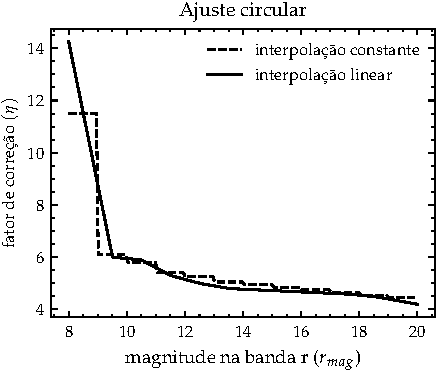
\includegraphics[width=0.51\linewidth]{notebooks/plots/correction_factor_circ.pdf}\hfill
  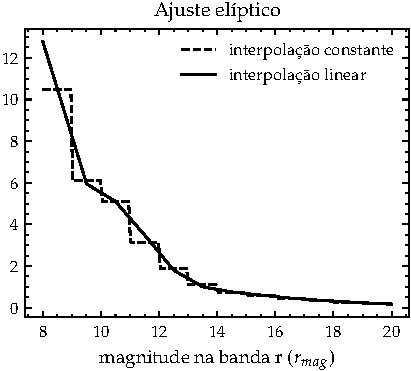
\includegraphics[width=0.48\linewidth]{notebooks/plots/correction_factor_ellip.pdf}
\end{figure}


O processo de ajuste do FoV é exemplificado nas figs. \ref{fig:fov-stamps-1} e \ref{fig:fov-stamps-2}. Nelas, são mostrados os ajustes de 12 galáxias, uma para cada intervalo de magnitude, tanto para o ajuste circular (primeiro método) quanto para o ajsute elíptico (segundo método). No ajuste circular, a circunferência indica o raio efetivo da galáxia escalonado pela função $\eta$. Analogamente, no ajuste elíptico, a elípse é obtida pelos parâmetros calculados nas eqs. \eqref{eq:b/a} e \eqref{eq:phi} escalonados pela função $\eta$, e o retângulo tracejado indica a caixa delimitadora da elípse, cujos limites são obtidos da eq. \eqref{eq:bb}. Em ambas as colunas, o quadrado branco indica o FoV calculado em cada caso, de acordo com as eqs. \eqref{eq:fov-circ} e \eqref{eq:fov-ellip}. As colunas ``corte circular'' e ``corte elíptico'' mostram as figuras finais após o ajuste pelo método do raio efetivo e da elipsidade complexa, respectivamente. A região vista nessas colunas é equivalente à região delimitada pelos quadrados brancos nas colunas de ajuste. Para comparação entre os métodos, ambas as colunas de ajuste possuem o mesmo FoV, definido manualmente para cada intervalo de magnitude.

Analisando os ajustes com o método do raio efetivo, notamos que há uma tendencia dessa abordagem subestimar o FoV de galáxias grandes, distorcidas ou de sistemas de galáxias, como mostra os Objetos 3 ao 6 da Fig. \ref{fig:fov-stamps-1} e o Objeto 7 da Fig. \ref{fig:fov-stamps-2}, além de sobre-estimar o FoV de galáxias menos brilhantes, como os Objetos 10 e 11 da Fig. \ref{fig:fov-stamps-2}. Por outro lado, o método da elípse pareceu mais consistente para determinação dos FoVs e por isso foi o método escolhido.

\begin{figure}[!ht]
  \centering
  \caption{Ajuste do campo de visão angular para $r_{mag}$ entre 8 e 13}
  \label{fig:fov-stamps-1}
  \includegraphics[width=0.99\linewidth]{notebooks/plots/stamps_crop_1.pdf}
\end{figure}

\begin{figure}[!ht]
  \centering
  \caption{Ajuste do campo de visão angular para $r_{mag}$ entre 14 e 19}
  \label{fig:fov-stamps-2}
  \includegraphics[width=0.99\linewidth]{notebooks/plots/stamps_crop_2.pdf}
\end{figure}








\subsection{Aquisição das Imagens}
\label{sec:aquisicao-stamps}

A aquisição dos pequenos recortes de imagens astronômicas centrados em objetos específicos (stamps) do Legacy Survey por meio do serviço Hips2Fits\footnote{\url{https://alasky.cds.unistra.fr/hips-image-services/hips2fits}} \cite{aladin}, do Strasbourg Astronomical Data Center\footnote{\url{https://cds.unistra.fr}} (CDS), envolve um processo meticuloso de coleta de imagens ajustadas para um grande número de galáxias. Considerando que os campos de visão (FOVs) de cada objeto foram previamente calculados para garantir que a área da galáxia ocupe uma proporção ideal na imagem, a aquisição pode então ser automatizada, eficiente e escalável. Para realizar essa aquisição em larga escala, que pode envolver milhões de galáxias, é fundamental utilizar uma arquitetura de paralelização eficiente, como o modelo de produtor-consumidor, combinada com mecanismos de controle de taxa de requisição, mostrado na Fig. \ref{fig:stamps-sequence}.

\begin{figure}[!ht]
  \centering
  \caption{Diagrama de sequência da arquisição das imagens}
  \label{fig:stamps-sequence}
  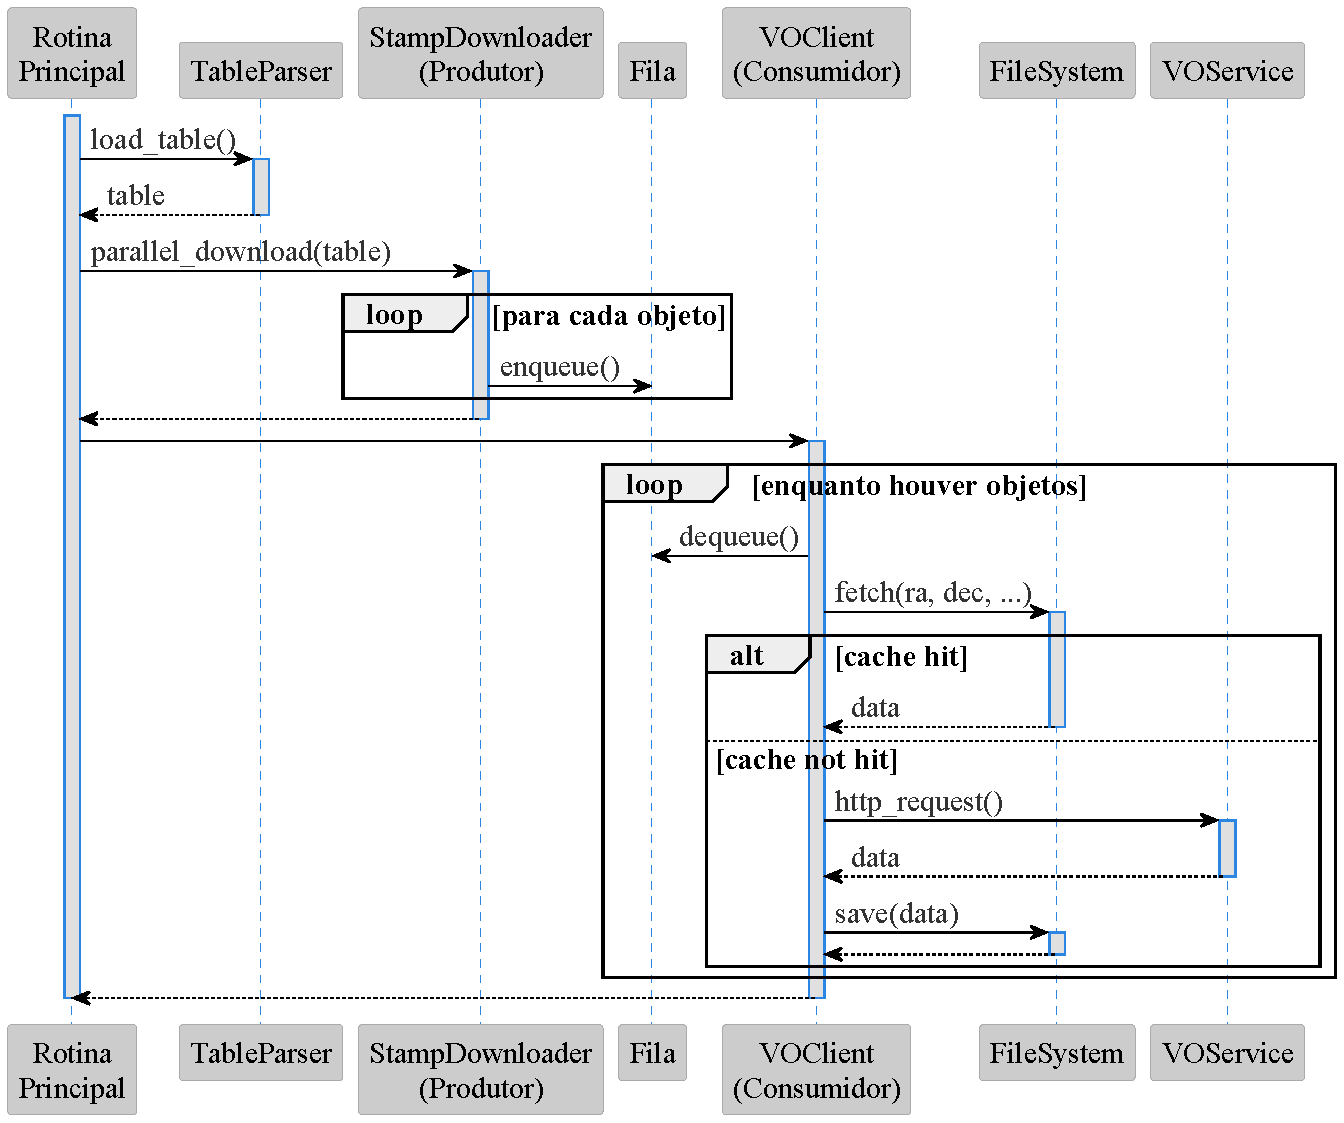
\includegraphics[width=\linewidth]{diagrams/plots/sequence.pdf}
\end{figure}


Inicialmente, o sistema é projetado em duas camadas principais: a camada de produtores, responsáveis por gerar as requisições de imagens para cada galáxia com seu respectivo FOV, e a camada de consumidores, encarregada de processar essas requisições e armazenar os stamps retornados. No caso de uma grande quantidade de objetos, é necessário implementar várias threads que operem de forma concorrente para maximizar o desempenho e a eficiência do sistema. Os produtores criam as requisições HTTP para o Hips2Fits, especificando os parâmetros de coordenadas do objeto (como RA e Dec) e o FOV calculado. Esses parâmetros garantem que a imagem adquirida seja adequada à análise morfológica planejada.

A arquitetura paralela é gerenciada com o uso de um semáforo, um mecanismo de controle de concorrência que limita o número de requisições simultâneas feitas ao servidor Hips2Fits. Esse semáforo é configurado de acordo com a taxa de requisição máxima permitida pelo servidor, evitando sobrecarga e bloqueios temporários ou permanentes impostos pelo controle de acesso ao servidor. O semáforo atua para que um número limitado de threads possa realizar requisições ao mesmo tempo; assim, ao alcançar o limite, novas requisições aguardam até que uma thread finalize seu processo e libere o semáforo para outra requisição.

Esse modelo de produtor-consumidor com controle de taxa de requisição não apenas respeita os limites de acesso do Hips2Fits, mas também assegura uma coleta eficiente e escalável. Como cada thread pode solicitar e processar imagens independentemente, o tempo total de execução é significativamente reduzido, permitindo a aquisição dos stamps para milhões de galáxias em um tempo viável. Essa abordagem de paralelização e controle de acesso torna o sistema robusto para grandes volumes de dados, possibilitando o processamento em lotes de imagens astronômicas de forma a atender à demanda de análise em larga escala na pesquisa astronômica.





\subsection{Descrição dos Conjuntos de Dados}
\label{sec:aquisicao-descricao}

Nesta Seção, é feita uma análise, de forma agregada, sobre as propriedades físicas das galáxias dos conjuntos de dados para garantir a coerência no treinamento do modelo.

\subsubsection{Conjuntos de Treinamento, Validação e Teste}
\label{sec:aquisicao-treinamento}

Garantir que os conjuntos de treinamento, validação e teste possuam distribuições similares de magnitude (Fig. \ref{fig:conjuntos_magr}) e campo de visão angular (Fig. \ref{fig:conjuntos_fov}) é crucial para o treinamento do modelo. Distribuições consistentes asseguram que o modelo seja exposto a dados representativos durante o treinamento, prevenindo vieses que poderiam comprometer sua capacidade de generalizar para novos dados. Magnitudes diferentes podem indicar variações no brilho dos objetos, influenciando os padrões visuais extraídos pelos modelos, enquanto campos de visão angulares distintos podem alterar o contexto espacial e os detalhes observados. Desequilíbrios entre esses conjuntos podem levar a discrepâncias na avaliação, onde métricas de desempenho no conjunto de teste não refletem a eficácia real do modelo em aplicações práticas.

\begin{figure}[!ht]
  \centering
  \caption{Distribuição da magnitude na banda r}
  \label{fig:conjuntos_magr}
  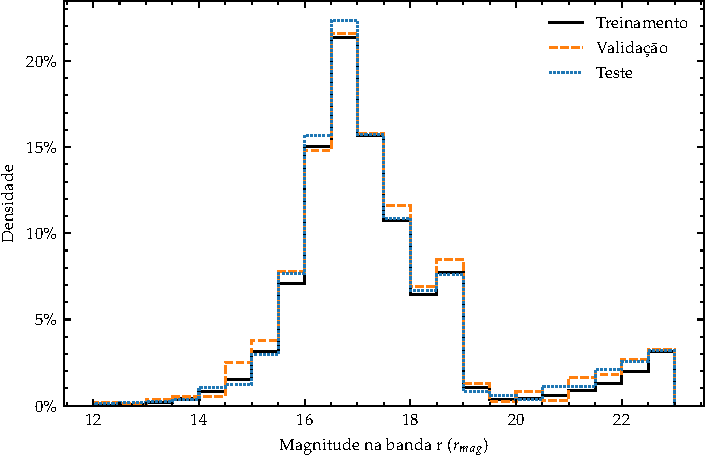
\includegraphics[width=\linewidth]{notebooks/plots/conjuntos_magr.pdf}
\end{figure}


\begin{figure}[!ht]
  \centering
  \caption{Distribuição do campo de visão angular}
  \label{fig:conjuntos_fov}
  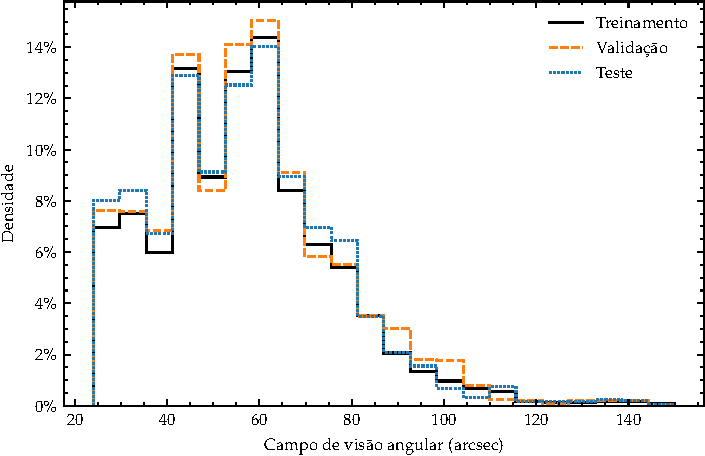
\includegraphics[width=\linewidth]{notebooks/plots/conjuntos_fov.pdf}
\end{figure}


\subsubsection{Conjunto de Inferência}
\label{sec:aquisicao-inferencia}

O conjunto de inferência é formado por aproximadamente 8 milhões de objetos. A Fig. \ref{fig:conjuntos_inferencia} mostra a distribuição espacial das galáxias, em que as cores codificam a densidade de galáxias em uma determinada região, conforme mostrado na escala.

\begin{figure}[!ht]
  \centering
  \caption{Área de cobertura espacial do conjunto de inferência}
  \label{fig:conjuntos_inferencia}
  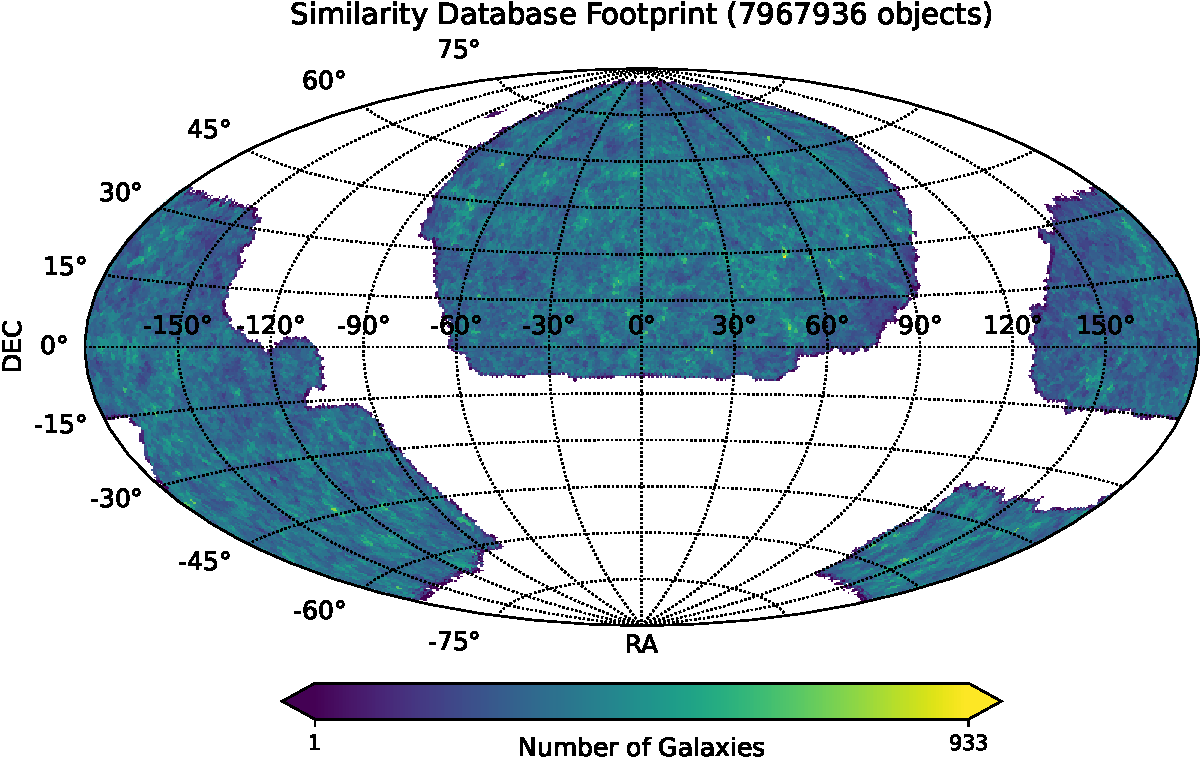
\includegraphics[width=\linewidth]{figures/similarity_footprint.pdf}
\end{figure}


Os conjuntos de treinamento e inferência utilizados neste trabalho, composto por 400 mil e 8 milhões de imagens obtidas do DESI Legacy Survey, respectivamente, possuem uma longa durabilidade científica devido às características intrínsecas do levantamento e ao tipo de observação realizada. Como um levantamento de campo profundo e não transiente, o Legacy Survey foca na captura de objetos celestes distantes e estáticos, como galáxias e aglomerados de galáxias, que não apresentam variações significativas em escalas temporais humanas. Esses objetos, frequentemente dominados por matéria escura, são fundamentais para o estudo da evolução cósmica e da distribuição de massa no universo em larga escala. A natureza estável dessas observações permite que os dados permaneçam relevantes por décadas, fornecendo uma base sólida para análises contínuas e complementares, à medida que novos modelos de aprendizado profundo e técnicas de análise de dados são desenvolvidos. Essa durabilidade é particularmente valiosa em um contexto científico onde as demandas computacionais e as abordagens metodológicas evoluem rapidamente, garantindo que o conjunto de inferência continue a contribuir para avanços na pesquisa astronômica e cosmológica.

Esta análise encerra a seção de descrição dos dados. A seguir, serão detalhados os métodos de aprendizado profundo utilizados para o treinamento do modelo.







\section{Modelo de Aprendizagem Profunda}
\label{sec:modelo}

Neste capítulo, será explicado sobre a preparação dos dados e como fizemos o aumento artificial dos dados para obter melhores resultados na avaliação dos modelos. Em seguida, descrevemos as redes convolucionais utilizadas: VGG, Inception Resnet, EfficientNet e DenseNet. Introduzimos o conceito de (\emph{Ensemble}) e descrevemos as técnicas usadas anteriormente e que fundamentaram nossas escolhas. Em seguida, apresentamos as principais definições das redes e parâmetros utilizados neste trabalho e por fim detalhamos como foram feitas as modelagens e treinamentos dos classificadores e do nosso meta-modelo.


\begin{figure}[!ht]
  \centering
  \caption{Fluxograma do treinamento do modelo}
  \label{fig:flow-modelo}
  \simpleflowdiagram{0.55}{
    Preparação das características (Seção \ref{sec:modelo-prep}),
    Aumento artificial de dados (Seção \ref{sec:modelo-dataaug}),
    Projeto da função custo (Seção \ref{sec:modelo-loss}),
    Hiperparâmetros (Seção \ref{sec:modelo-hp}),
    Treinamento (Seção \ref{sec:modelo-treinamento}),
    Métricas de Avaliação (Seções \ref{sec:metricas-votos} e \ref{sec:metricas-sim})
  }
\end{figure}


\subsection{Preparação das Características}
\label{sec:modelo-prep}
A preparação dos dados é a etapa intuitivamente subsequente, após a aquisição (Seção \ref{sec:aquisicao}). Nessa subseção, é discutido o processamento e codificação das catacterísticas de entrada (Seção \ref{sec:modelo-prep-input}) e dos rótulos (Seção \ref{sec:modelo-prep-labels}).


\subsubsection{Preparação das Características de Entrada}
\label{sec:modelo-prep-input}
As características de entrada do modelo são as imagens do Legacy Survey DR10 (Seção \ref{sec:legacy}), obtidas pelo método descrito na Seção \ref{sec:aquisicao-stamps}. Uma etapa importante da seleção dessas características é o ajuste do campo de visão (FoV) de cada imagem. Esse ajuste determina a porcentagem que a galáxia ocupa na imagem. Visto que os píxeis referentes às galáxias são as únicas características de interesse, esse ajuste é fundamental para garantir o desempenho do modelo. Como o FoV deve ser especificado previamente, no momento da aquisição da imagem, essa etapa de ajuste do FoV já foi discutida na Seção \ref{sec:aquisicao-fov}.

O primeiro pré-processamento feito é a soma pixel a pixel no eixo dos canais RGB, produzindo uma imagem em níveis de cinza, com um único canal. Dessa forma, é mantida apenas a informação estrutural de cada galáxia. Em seguida, é feita uma normalização usando a média e o desvio padrão do lote (\texttt{BatchNormalization}).


\subsubsection{Preparação dos Rótulos}
\label{sec:modelo-prep-labels}
Os rótulos são formados pelas contagens das respostas dos voluntários do GalaxyZoo para cada galáxia. Isto é, os votos são agregados em relação a cada galáxia. As contagens de votos de cada alternativa são arranjadas na forma de vetor e os votos de diferentes campanhas são concatenados em um único vetor de votos, que é considerado o valore de referência para a estimativa das contagens de votos durante o treinamento do modelo.





\subsection{Aumento Artificial de Dados}
\label{sec:modelo-dataaug}

\begin{figure*}[!ht]
  \centering
  \caption{Aumento artificial dos dados}
  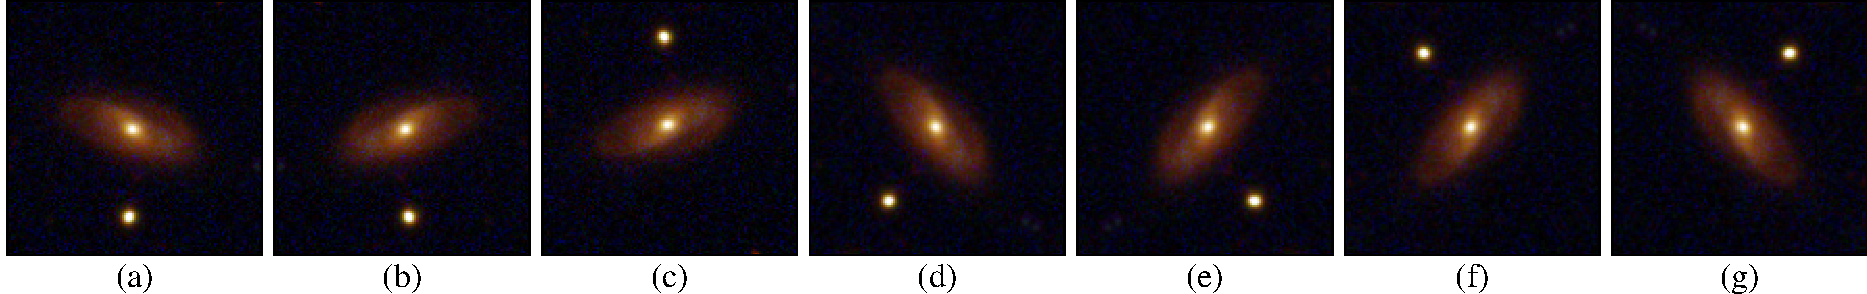
\includegraphics[width=\linewidth]{figures/dataaug.pdf}
  \legend{Exemplo do aumento artificial de dados em uma imagem original, mostrada no painel (a). Os painéis (b), (c), (d), (e), (f) e (g) contêm os resultados da eq. \eqref{eq:final-transformation} substituindo $M$ por diferentes combinações das transformações das eqs. \eqref{eq:aug-rot}, \eqref{eq:aug-h} e \eqref{eq:aug-v}. Em (b) $M = V$, em (c) $M = H$, em (d) $M = R(30\degree)$, em (e) $M = V R(30\degree)$, em (f) $M = H R(30\degree)$ e em (g) $M = H V R(30\degree)$.}
  \label{fig:dataaug}
\end{figure*}

Aumento artificial de dados \cite{Larry1996} é a aplicação de transformações afins nas imagens do conjunto de treinamento, por exemplo rotação, reflexão, translação e mudança de escala. As matrizes das eqs. \eqref{eq:aug-rot}, \eqref{eq:aug-h} e \eqref{eq:aug-v} definem as transformações usadas.


\begin{equation}\label{eq:aug-rot}
  R(\theta) =
  \begin{bmatrix}
    \cos(\theta) & -\sin(\theta) & 0 \\
    \sin(\theta) & \cos(\theta)  & 0 \\
    0            & 0             & 1
  \end{bmatrix}
\end{equation}


\begin{equation}\label{eq:aug-h}
  H =
  \begin{bmatrix}
    1 & 0  & 0 \\
    0 & -1 & 0 \\
    0 & 0  & 1
  \end{bmatrix}
\end{equation}


\begin{equation}\label{eq:aug-v}
  V =
  \begin{bmatrix}
    -1 & 0 & 0 \\
    0  & 1 & 0 \\
    0  & 0 & 1
  \end{bmatrix}
\end{equation}


onde $R(\theta)$ é a transformação rotação por um ângulo $\theta$,
$H$ é a transformação reflexão horizontal e $V$ é a transformação reflexão vertical, nas eqs. \eqref{eq:aug-rot}, \eqref{eq:aug-h} e \eqref{eq:aug-v}, respectivamente.

Seja $M$ a matriz das transformações combinadas, $(x, y)$ a coordenada do píxel da imagem original e $(x^*, y^*)$ a coordenada transformada do píxel, as transformações nas imagens são feitas remapeando as coordenadas dos píxeis originais aplicando uma combinação das matrizes das eqs. \eqref{eq:aug-rot}, \eqref{eq:aug-h} e \eqref{eq:aug-v} em cada píxel da imagem original usando a equação \eqref{eq:final-transformation}, onde $(t_x, t_y)$ é a coordenada do centro da imagem e as matrizes ao redor de $M$ são as matrizes translação. Isso é feito para que a transformação $M$ tenha o centro da imagem como ponto de simetria.

\begin{align} \label{eq:final-transformation}
  \begin{bmatrix}
    x^* \\
    y^* \\
    1
  \end{bmatrix}
  =
  \begin{bmatrix}
    1 & 0 & t_x \\
    0 & 1 & t_y \\
    0 & 0 & 1
  \end{bmatrix}
  \ M\
  \begin{bmatrix}
    1 & 0 & -t_x \\
    0 & 1 & -t_y \\
    0 & 0 & 1
  \end{bmatrix}
  \begin{bmatrix}
    x \\
    y \\
    1
  \end{bmatrix}
\end{align}

Além disso, ainda é aplicada uma interpolação bilinear como \emph{anti-aliasing} \cite{aliasing,bilinear}. Durante o treinamento da rede, novas imagens de entrada são geradas a cada época a partir da transformação das imagens originais. A Figura \ref{fig:dataaug} mostra a imagem original, no painel (a), e diversas transformações, nos demais painéis, aplicadas substituindo $M$ da equação \eqref{eq:final-transformation} por combinações (multiplicação matricial) das transformações das eqs. \eqref{eq:aug-rot}, \eqref{eq:aug-h} e \eqref{eq:aug-v}. Tais transformações não mudam a interpretação da classe da imagem original, pois o espaço visual é invariante a elas. Logo, o objetivo de aplicar estas transformações nas imagens de entrada da rede é deixar que o algorítmo infira tal invariância, criando, assim, uma ``noção'' do espaço visual, o que resulta no aumento do potencial de generalização da rede \cite{Simard2003,CholletBook}. Frequentemente são relatados bons resultados com o uso desta técnica \cite{EfficientNetEx01,EfficientNetEx02,CNNEx04}, principalmente quando existe grande similaridade entre as classes.






% \subsection{Preparação dos dados}
% \label{section:preparacao}

% O pré-processamento é a preparação das imagens para serem usadas pelo modelo, ou seja, é a transformação dos dados não processados em dados prontos para entrada na rede. Isso envolve representar as imagens por matrizes multidimensionais, onde cada elemento da matriz representa um pixel da imagem, e aplicar algumas transformações, especificadas a seguir.

% \subsubsection{Agrupamento das bandas para confecção das imagens RGB}

% Como as imagens do S-PLUS foram obtidas em 12 bandas fotométricas (listadas em \cite{splus}), para representá-las no sistema de cor RGB fizemos o seguinte mapeamento: em R colocamos as 4 bandas vermelhas r\_SDSS, i\_SDSS, J0861 e z, em G as bandas g\_SDSS J0515 e J0660 e em B as cinco bandas mais azuis u\_JAVA, J0373, J0395, J0410 e J0430 (as características destes filtros são dadas na Tabela 1 de \cite{splus}). Na combinação de bandas em cada canal, foi feita uma soma simples dos valores dos píxeis. Depois de reduzidas a três bandas, as imagens são usadas como entrada do programa Trilogy\cite{coe2012clash}\footnote{\url{https://www.stsci.edu/~dcoe/trilogy/Intro.html}}.

% \subsubsection{ImageNet}

% Como já mostrado em trabalhos anteriores, a inicialização dos pesos provenientes de uma rede pré-treinada usando a base de dados \emph{ImageNet}\footnote{\url{http://www.image-net.org/}} traz uma grande melhoria na precisão dos resultados da classificação. Essa base de dados possui milhões de imagens de objetos do cotidiano e já foi utilizada especificamente para a classificação de objetos astronômicos (veja por exemplo \cite{bom2021}), com excelentes resultados.

% O uso deste dataset para pré-treinamento respeitou o pré-processamento utilizado originalmente pelos autores de cada rede, este procedimento este foi crucial para garantir um fit competitivo, isto é, no \textit{benchmarking} original destas redes para os dados da \emph{ImageNet}. Para a rede VGG16 (Seção \ref{section:vgg}), a ordem das bandas foi trocada de RGB para BGR, e cada banda foi centrada em zero em relação à \emph{ImageNet}, sem escalonamento, ou seja, os píxeis de cada banda tiveram o valor da média da respectiva banda \emph{ImageNet} subraído. Para a rede InceptionResNetV2 (Seção \ref{section:inceptionresnetv2}), os píxeis de entrada foram escalonados entre -1 e 1 em relação a amostra de treino. Para a rede EfficientNet (Seção \ref{section:efficientnet}), os píxeis de entrada foram escalonados entre 0 e 1 em relação à amostra de treino. E, para a rede DenseNet (Seção \ref{section:densenet}), os píxeis de entrada foram escalonados entre 0 e 1 e cada banda foi padronizada em relação à \emph{ImageNet}, isto é, os píxeis de cada banda tiveram o valor da média subtraído e o resultado foi dividido pelo desvio padrão da distribuição da respectiva banda da \emph{ImageNet}.

% \begin{figure*}[!ht]
%   \centering
%   \includegraphics[width=\textwidth]{figures/arch.pdf}
%   \caption{Diagrama que descreve a arquitetura da rede. Da esquerda para a direita, as 12 imagens de cada banda são agrupadas em uma única imagem RGB (Seção \ref{section:preparacao}), que é a entrada dos classificadores indidviduais. Estes classificadores (Seção \ref{section:classificador}) têm a função de extrair características visuais da imagem e retornar a probabilidade de ser elíptica ou espiral. O meta-modelo (Seção \ref{section:meta-modelo}) tem a função de combinar as predições dos classificadores em uma única predição final mais robusta.}
%   \label{fig:arch}
% \end{figure*}






\subsection{Função de Custo}
\label{sec:modelo-loss}


\subsubsection{Distribuição Multinomial}
\label{sec:modelo-multi}

A distribuição multinomial \cite{distbook-multinomial} é uma generalização da distribuição binomial \cite{distbook-binomial} que descreve o comportamento de um experimento discreto onde cada tentativa resulta em um de $k$ possíveis resultados mutuamente exclusivos.

Supondo que um experimento é repetido $n$ vezes, e que a probabilidade de cada resultado específico $i$, para $i=1,2,\dots,k$, seja $p_i$, com $\sum_{i=1}^k p_i = 1$. A distribuição multinomial caracteriza a probabilidade conjunta de observar cada um dos $k$ resultados um número específico de vezes ($x_1, x_2,\dots, x_k$), onde $\sum_{i=1}^k x_i = n$. A função de probabilidade associada é definida pela eq. \eqref{eq:multinomial}, onde \( x_i \geq 0 \) representa a contagem de ocorrências para cada categoria \( i \).

\begin{equation}\label{eq:multinomial}
  P(X_1 = x_1, X_2 = x_2, \dots, X_k = x_k) = \frac{n!}{x_1! x_2! \cdots x_k!} \prod_{i=1}^k p_i^{x_i}
\end{equation}

A distribuição multinomial \cite{seber2015-multi} é amplamente utilizada em aplicações de aprendizado de máquina e estatística, como na modelagem da transmissão de Dengue \cite{wang2025}, na predição de cotação de mercado \cite{nevasalmi2020} e na análise de tráfego aéreo \cite{torres2023}. Uma de suas principais aplicações é em modelagem de eventos categóricos \cite{kibriya2004,luo2021}. Por exemplo, em tarefas de classificação multiclasse, onde o objetivo é prever a probabilidade de uma amostra pertencer a uma entre várias categorias, a distribuição multinomial é usada para modelar a saída do modelo. Um exemplo prático é o uso em algoritmos como o Naive Bayes Multinomial \cite{kalcheva2023,jiang2016}, amplamente empregado em problemas de classificação de texto \cite{odeh2022,kan2005}, como análise de sentimentos \cite{saravanan2023} e categorização de documentos. Neste contexto, as palavras em um documento são tratadas como eventos que seguem uma distribuição multinomial.

% Outra aplicação significativa é no modelamento de linguagens probabilísticas, como em modelos n-grama usados para processamento de linguagem natural (NLP). Nesses modelos, a distribuição multinomial é usada para representar a probabilidade de coocorrência de palavras em sequência. Além disso, na estimação de tópicos em conjuntos de documentos, como no algoritmo Latent Dirichlet Allocation (LDA), a distribuição multinomial é usada para modelar a distribuição de palavras em tópicos e tópicos em documentos.

% No campo de aprendizado profundo, a distribuição multinomial aparece em camadas de saída de redes neurais voltadas para classificação multiclasse, onde a função softmax é usada para transformar as saídas da rede em probabilidades que seguem uma distribuição multinomial. Esse uso é especialmente prevalente em problemas como reconhecimento de imagens e detecção de objetos.

% Por fim, a distribuição multinomial também desempenha um papel importante em amostragem e inferência estatística. Em métodos como amostragem Gibbs e Markov Chain Monte Carlo (MCMC), é comum gerar amostras a partir de distribuições multinomiais para explorar o espaço de parâmetros em modelos probabilísticos complexos.


\subsubsection{Distribuição de Dirichlet}
\label{sec:modelo-dir}

A distribuição Dirichlet \cite{distbook-dirichlet} é uma distribuição de probabilidade multivariada contínua definida no simplex \( k \)-dimensional, sendo uma generalização da distribuição Beta \cite{distbook-beta} para múltiplas dimensões. Ela é frequentemente utilizada para modelar distribuições de probabilidade sobre proporções, em que cada elemento do vetor de variáveis aleatórias representa uma fração de um todo e, portanto, suas somas totalizam 1.

Dada uma variável aleatória \( \vec{X} = (X_1, X_2, \dots, X_k) \) que segue uma distribuição Dirichlet com parâmetro de concentração \( \vec{\alpha} = (\alpha_1, \alpha_2, \dots, \alpha_k) \) para uma quantidade $k$ de categorias, a função de densidade de probabilidade é definida pela eq. \eqref{eq:dirichlet}, onde \( B(\vec{\alpha}) \) é a função beta multivariada, definida na eq. \eqref{eq:dirichlet-B}, e \( \Gamma(\cdot) \) representa a função gama \cite{distbook-gamma}. O parâmetro \( \alpha_i \) controla a concentração da probabilidade ao redor das categorias: valores maiores de \( \alpha_i \) indicam maior densidade de probabilidade associada à categoria correspondente.

\begin{equation}\label{eq:dirichlet}
  P(\vec{X} | \vec{\alpha}) = \frac{1}{B (\vec{\alpha})} \prod_{i=1}^k X_i^{\alpha_i - 1}
\end{equation}

\begin{equation}\label{eq:dirichlet-B}
  B(\vec{\alpha}) = \frac{\prod_{i=1}^k \Gamma(\alpha_i)}{\Gamma\left(\sum_{i=1}^k \alpha_i\right)}
\end{equation}


Em aprendizado de máquina, a distribuição Dirichlet possui aplicações importantes em problemas que envolvem modelagem de distribuições de probabilidade sobre categorias. Um exemplo clássico é na modelagem de misturas probabilísticas, como no algoritmo Latent Dirichlet Allocation (LDA; \citealp{lda}), amplamente utilizado para análise de tópicos em grandes corpora de texto \cite{jelodar2019}. No LDA, a distribuição Dirichlet é usada como uma distribuição a priori para representar a probabilidade de tópicos em documentos e a probabilidade de palavras em tópicos, fornecendo uma forma eficiente de capturar relações semânticas latentes \cite{canini2009}.

% Além disso, a distribuição Dirichlet é usada em inferência bayesiana, especialmente como conjugado da distribuição multinomial. Em tarefas como classificação multiclasse, a combinação da distribuição Dirichlet com a multinomial permite a atualização eficiente das probabilidades a priori para a modelagem de eventos categóricos. Esse mecanismo é essencial em algoritmos de aprendizado supervisionado que se baseiam em pressupostos probabilísticos, como o Naive Bayes Multinomial.

% Outro campo de aplicação da distribuição Dirichlet é o **aprendizado de misturas**, onde modelos como o Dirichlet Process Mixture Model (DPMM) usam essa distribuição para lidar com dados agrupados, mas com um número potencialmente infinito de clusters. Essa característica é particularmente útil em problemas não supervisionados, onde o número de classes ou clusters não é conhecido a priori.

% Na **simulação e geração de dados sintéticos**, a distribuição Dirichlet é frequentemente empregada para gerar distribuições de probabilidades em modelos de simulação. Por exemplo, em aprendizado por reforço, ela pode ser usada para modelar incertezas nas probabilidades de transição entre estados em ambientes estocásticos.

% Por fim, a distribuição Dirichlet também desempenha um papel em métodos de regularização. Em problemas de otimização envolvendo distribuições de probabilidades, ela pode ser usada para impor uma estrutura probabilística bem definida, evitando soluções degeneradas ou com concentração excessiva de probabilidades em poucas categorias.

% Em resumo, a distribuição Dirichlet é uma ferramenta central para modelar proporções e distribuições categóricas em múltiplas áreas do aprendizado de máquina, oferecendo uma base teórica sólida para lidar com problemas envolvendo incertezas e relações probabilísticas complexas.




\subsubsection{Distribuição Dirichlet-Multinomial}
\label{sec:modelo-dir-multi}

A distribuição Dirichlet-multinomial \cite{distbook-dirichlet} é uma distribuição de probabilidade discreta que combina as propriedades da distribuição multinomial (Seção \ref{sec:modelo-multi}) e da distribuição Dirichlet (Seção \ref{sec:modelo-dir}). Ela é usada para modelar processos em que as probabilidades das categorias em uma distribuição multinomial são, elas mesmas, amostras de uma distribuição Dirichlet. Isto é, a distribuição Dirichlet é usada como distribuição a priori para estimar os parâmetros da distribuição multinomial. Essa estrutura permite incorporar incertezas sobre as probabilidades subjacentes das categorias.

Formalmente, dado um vetor \( \vec{\theta} = (\theta_1, \theta_2, \dots, \theta_k) \) de probabilidades categóricas que segue uma distribuição Dirichlet com parâmetro \( \vec{\alpha} = (\alpha_1, \alpha_2, \dots, \alpha_k) \), e uma distribuição multinomial condicional sobre \( \vec{\theta} \), a probabilidade conjunta da distribuição Dirichlet-multinomial é expressa na eq. \eqref{eq:dirichlet-multinomial}, onde \( n = \sum_{i=1}^k x_i \) é o número total de experimentos, e \( x_i \) representa o número de ocorrências da \( i \)-ésima categoria.

\begin{equation}\label{eq:dirichlet-multinomial}
  P(X_1 = x_1, X_2 = x_2, \dots, X_k = x_k) = \frac{\Gamma\left(\sum_{i=1}^k \alpha_i\right)}{\Gamma\left(\sum_{i=1}^k \alpha_i + n\right)} \prod_{i=1}^k \frac{\Gamma(x_i + \alpha_i)}{\Gamma(\alpha_i) \, x_i!}
\end{equation}




\subsubsection{Função de Custo e Função de Perda}
\label{sec:modelo-loss-cost}

A função de perda (\emph{loss function}) e a função de custo (\emph{cost function}) têm papéis relacionados, mas distintos. A primeira avalia o erro do modelo em uma única amostra, medindo a discrepância entre a predição do modelo e o valor esperado. Já a segunda, é uma agregação da primeira, geralmente calculada como a média ou soma das perdas sobre todo o conjunto de treinamento, representando o desempenho global do modelo. %Isto é, enquanto a loss function opera em nível de exemplo individual, a cost function fornece uma visão geral para otimizar o modelo durante o treinamento.

% A escolha da função de perda possui impacto direto na capacidade preditiva do modelo. Por isso, escolhemos uma função de custo

% As informações morfológicas sobre as galáxias são obtidas pelo projeto GalaxyZoo, que consistem nos votos de voluntários para diversas perguntas sobre suas características visuais, como a orientação espacial, a presença de bojo, a quantidade de braços espirais, etc. Então, considerando a origem dos dados, a distribuição Dirichlet-multinomial (Seção \ref{sec:modelo-dir-multi}) foi escolhida como função de custo.

A função de perda de uma pergunta $q$ é calculada a partir da distribuição Dirichlet-Multinomial, conforme a eq. \eqref{eq:loss}.

\begin{equation}\label{eq:loss}
  \mathcal{L}_q = \int\text{Multi}(\vec{k}|\vec{\rho}, N) \text{Dirichlet}(\vec{\rho}|\vec{\alpha})d\vec{\rho}
\end{equation}

Já o valor da perda de um exemplo é a soma das perdas de cada questão $q$, conforme a eq. \eqref{eq:log_loss}.

\begin{equation}\label{eq:log_loss}
  \log \mathcal{L} = \sum_q \mathcal{L}_q(\vec{k_q}, N_q, \vec{f_q^w})
\end{equation}

Existem duas formas recorrentes de agregar as perdas dos exemplos para calcular o custo total do modelo: calcular a soma  ou a média. Nesse trabalho, a função de custo é definda como a soma de todas as perdas de cada exemplo do conjunto de dados, conforme eq. \eqref{eq:cost}.

\begin{equation}\label{eq:cost}
  J = \sum_i \log \mathcal{L}_i
\end{equation}


% ### Propriedades e Intuição
% A distribuição Dirichlet-multinomial é uma extensão prática da distribuição multinomial porque incorpora variabilidade adicional na estimativa das probabilidades \( \boldsymbol{\theta} \). Isso a torna ideal para modelar dados categóricos onde há incerteza ou variabilidade na distribuição subjacente. Como tal, ela é frequentemente descrita como uma multinomial com parâmetros aleatórios seguindo uma Dirichlet.

% ### Aplicações em Aprendizado de Máquina
% No campo de aprendizado de máquina, a distribuição Dirichlet-multinomial possui aplicações significativas em **modelagem probabilística** e **inferência bayesiana**. Uma de suas utilizações mais comuns é na modelagem de fenômenos categóricos em que a frequência das categorias varia entre diferentes conjuntos de dados ou instâncias.

% #### 1. **Latent Dirichlet Allocation (LDA)**
% Na análise de tópicos, a Dirichlet-multinomial é usada para modelar a distribuição das palavras em documentos. Cada documento é tratado como uma realização de uma multinomial, cujas probabilidades de categorias (palavras) são amostras de uma Dirichlet. Essa abordagem permite capturar as variações de distribuição de palavras entre tópicos, sendo central para algoritmos como o **Latent Dirichlet Allocation (LDA)**, amplamente utilizado em **processamento de linguagem natural**.

% #### 2. **Inferência Bayesiana em Classificação Multiclasse**
% A Dirichlet-multinomial é o modelo conjugado da distribuição multinomial em inferência bayesiana. Em problemas de **classificação multiclasse**, ela é usada para modelar a incerteza nas estimativas das probabilidades das classes, particularmente em cenários de aprendizado supervisionado onde os dados de treinamento são limitados.

% #### 3. **Modelagem de Contagens e Variabilidade**
% Problemas que envolvem dados de contagem, como análise de redes sociais, preferências de usuários ou frequências de eventos em sistemas distribuídos, frequentemente apresentam superdispersão (variância maior que a média). A Dirichlet-multinomial é adequada para modelar essa superdispersão, fornecendo uma alternativa robusta à multinomial tradicional.

% #### 4. **Misturas de Modelos e Clusterização**
% Na clusterização, especialmente em métodos baseados em misturas, como o **Dirichlet Process Mixture Models (DPMM)**, a Dirichlet-multinomial pode ser usada para modelar distribuições de contagens em diferentes clusters. Esse uso é especialmente relevante em problemas de agrupamento não supervisionado.

% #### 5. **Geração de Dados Sintéticos**
% A distribuição Dirichlet-multinomial também é amplamente utilizada para gerar dados categóricos sintéticos que incorporam incertezas ou variabilidades realistas, sendo valiosa em experimentos controlados e validações de algoritmos.

% ### Conclusão
% A distribuição Dirichlet-multinomial é uma ferramenta poderosa para modelar processos categóricos que exibem variabilidade nas probabilidades subjacentes. Sua capacidade de capturar incertezas intrínsecas torna-a essencial em uma ampla gama de aplicações, especialmente na modelagem de tópicos, inferência bayesiana e análise de dados de contagem. No aprendizado de máquina, ela desempenha um papel central ao lidar com problemas onde a variabilidade das distribuições subjacentes é uma característica fundamental dos dados.




\subsection{Hiperparâmetros}
\label{sec:modelo-hp}

Nesta seção descrevemos as definições dos principais conceitos, no contexto de deep learning, que serão úteis para o entendimento dos métodos aqui utilizados. A função de ativação, função de custo, o otimizador, o learning rate, o número de épocas, além do número de camadas dos modelos, são importantes parâmetros responsáveis pela contrução do modelo definido a seguir.

\begin{description}
  \item[Função de ativação] \hfill \\
        A função de ativação é responsável por adicionar não-linearidade à rede. Sem ela, a saída de uma camada seria apenas uma transformação linear dos dados de entrada e a rede não seria beneficiada pelo empilhamento de diversas camadas lineares, pois isso não aumentaria o espaço de hipóteses. Logo, a função de ativação viabiliza representações mais complexas da rede, uma vez que define a complexidade de um modelo e, consequentemente, sua capacidade de generalização \cite{CholletBook}. Neste trabalho, a função $\textrm{ReLU}(x) := \textrm{max}(0, x)$ é usada nas camadas densas dos classificadores, a equação tangente hiperbólica é usada nas camadas densas do meta-modelo e a função Softmax \cite{Bridle1990} foi usada na última camada, tanto dos classificadores quanto do meta-modelo.

  \item[Otimizador] \hfill \\
        O otimizador é um algorítmo iterativo com objetivo de minimizar a função de custo. Uma escolha típica é o método de gradiente descente e suas demais variações. Este tipo de algoritmo tem um parâmetro livre relacionado ao passo da iteração conhecido como taxa de aprendizado ou \textit{learning rate}. Neste trabalho foram testados diversos algoritmos considerados como estado-da-arte dos otimizadores como Adam \cite{Adam}, NAdam \cite{NAdam}, RAdam \cite{RAdam} e RMSprop \cite{RMSprop}.

  \item[Número de Épocas] \hfill \\
        O Número de épocas se referem a quantidade de vezes que o dataset de treino foi utilizado completamente no processo de otimização iterativa da função de custo. Um número de épocas adequado é necessário para que a função de custo seja minimizada.

  \item[Tamanho do Batch] \hfill \\
        O processo de otimização acontece em batches, cada iteração para minimizar a função custo é realizada com um número fixo de amostras, quando todas as amostras de treino são utilizadas se completa uma época.

  \item[Unidades de neurônios na última camada]
        \hfill \\
        A última camada da rede antes da camada de saída é responsável por condensar toda a informação extraída da rede para o processo de classificação final. Por esta razão, a quantidade de neurônios nessa camada pode ser particularmente sensível para a performance da rede. Neste trabalho utilizamos diferentes valores de neurônios para encontrar a quantidade que pode gerar a melhor performance.

  \item[Dropout]
        \hfill \\
        \emph{Dropout} \cite{dropout} é uma técnica de regularização muito utilizada em redes neurais por seu bom desempenho e baixo custo computacional. Aplicar esta regularização em uma camada consiste em eliminar aleatoriamente uma taxa dos neurônios de saída desta camada durante o treinamento, sendo geralmente escolhido um valor entre 0.2 e 0.5 para esta taxa \cite{CholletBook}.
\end{description}












\subsection{Arquitetura de Rede Neural}
\label{sec:arch}

\subsubsection{Visual Geometry Group Networks}
\label{sec:vgg}
A família de arquiteturas Visual Geometry Group Networks (VGGNets) \cite{VGG16} foi criada durante a competição de classificação de imagens \textit{Large Scale Visual Recognition Challenge} \cite{ILSVRC15}. Ela se destaca por estar entre as primeiras redes a adotar, com sucesso, o escalamento em profundidade (quantidade de camadas) para aumentar o desempenho na classificação de imagens usando redes convolucionais. Neste trabalho, consideramos a arquitetura VGG16, que já foi usada em diversas tarefas de classificação, como a classificação de software malicioso \cite{VGG16Ex01}, de plantas \cite{VGG16Ex02} e de tumores cerebrais \cite{VGG16Ex03}.

\subsubsection{InceptionResNetV2}
\label{sec:inceptionresnetv2}
A arquitetura InceptionResNetV2 \cite{InceptionResNetv2} usa os blocos Inception, que são convoluções fatorizadas, introduzidos em \cite{Inception}, motivada pela construção de redes mais profundas com um menor custo computacional e menor overfitting, com a adição de conexões residuais \cite{ResNet} motivada pelo problema de dissipação do Gradiente (\textit{vanishing gradients}). Isso permite treinar redes profundas com maior acurácia e mais rápido. Esta arquitetura já foi usada, por exemplo, para classificação de imagens de satélite \cite{InceptionResNetV2Ex01}, de ultrasonografia \cite{InceptionResNetV2Ex02} e de células cancerígenas \cite{InceptionResNetV2Ex03}.

\subsubsection{EfficientNet}
\label{sec:efficientnet}
A arquitetura EfficientNet \cite{EfficientNet} foi desenvolvida como uma resposta à questão de como escalar modelos de convolução. Foram considerados três diferentes aspectos: profundidade, largura e resolução da imagem de entrada. Em vez de dimensionar cada aspecto manualmente, o modelo implementa um escalonamento composto que equilibra os aspectos para obter melhor desempenho, com isso a rede consegue uma alta acurácia usando muito menos parâmtros e operações de ponto flutuante por segundo (\emph{FLOPS}). Esta rede já foi usada na classificação de doenças em vegetais \cite{EfficientNetEx03}, eletrocardiogramas \cite{EfficientNetEx01} e cristalização de proteínas \cite{EfficientNetEx02}.

\subsubsection{DenseNet}
\label{sec:densenet}
A rede DenseNet \cite{DenseNet} também usa conexões residuais que conectam cada camada a todas as outras camadas seguintes, o que reduz ainda mais o número de parâmetros na rede sem perda significativa da precisão. O uso desta rede incluem predição do mapa de contato de proteínas \cite{DenseNetEx02}, classificação de músicas \cite{DenseNetEx05}, câncer de mama \cite{DenseNetEx01} e esclerose múltipla \cite{DenseNetEx03}.


\subsubsection{Escolha da Arquitetura}
\label{sec:escolha-arch}
Todas as arquiteturas convolucionais mencionadas nessa seção foram testadas e a arquitetura que teve melhor desempenho na predição dos votos dos voluntários foi escolhida. O processo de treinamento e avaliação está descrito na seção seguinte.



\subsection{Treinamento}
\label{sec:modelo-treinamento}

O treinamento de modelos de aprendizado profundo é um processo complexo que envolve a escolha de uma arquitetura adequada e a definição de hiperparâmetros que otimizem o desempenho do modelo em um conjunto de dados específico. A técnica de treinamento automatizado (AutoML; \citealp{automl}), mostrada na Fig. \ref{fig:treinamento}, facilita esse processo de seleção de hiperparâmetros e configurações de treinamento. Neste trabalho, foi utilizada uma abordagem que se mostrou eficaz nesse contexto: os algoritmos Multi-Objective Tree-structured Parzen Estimator (MOTPE; \citealp{motpe}) e HyperBand (HB; \citealp{hyperband}), disponíveis na biblioteca Optuna\footnote{\url{https://optuna.org}} \cite{optuna}, para a otimização de múltiplos objetivos simultaneamente.

\begin{figure}[!ht]
  \centering
  \caption{Treinamento do modelo}
  \label{fig:treinamento}
  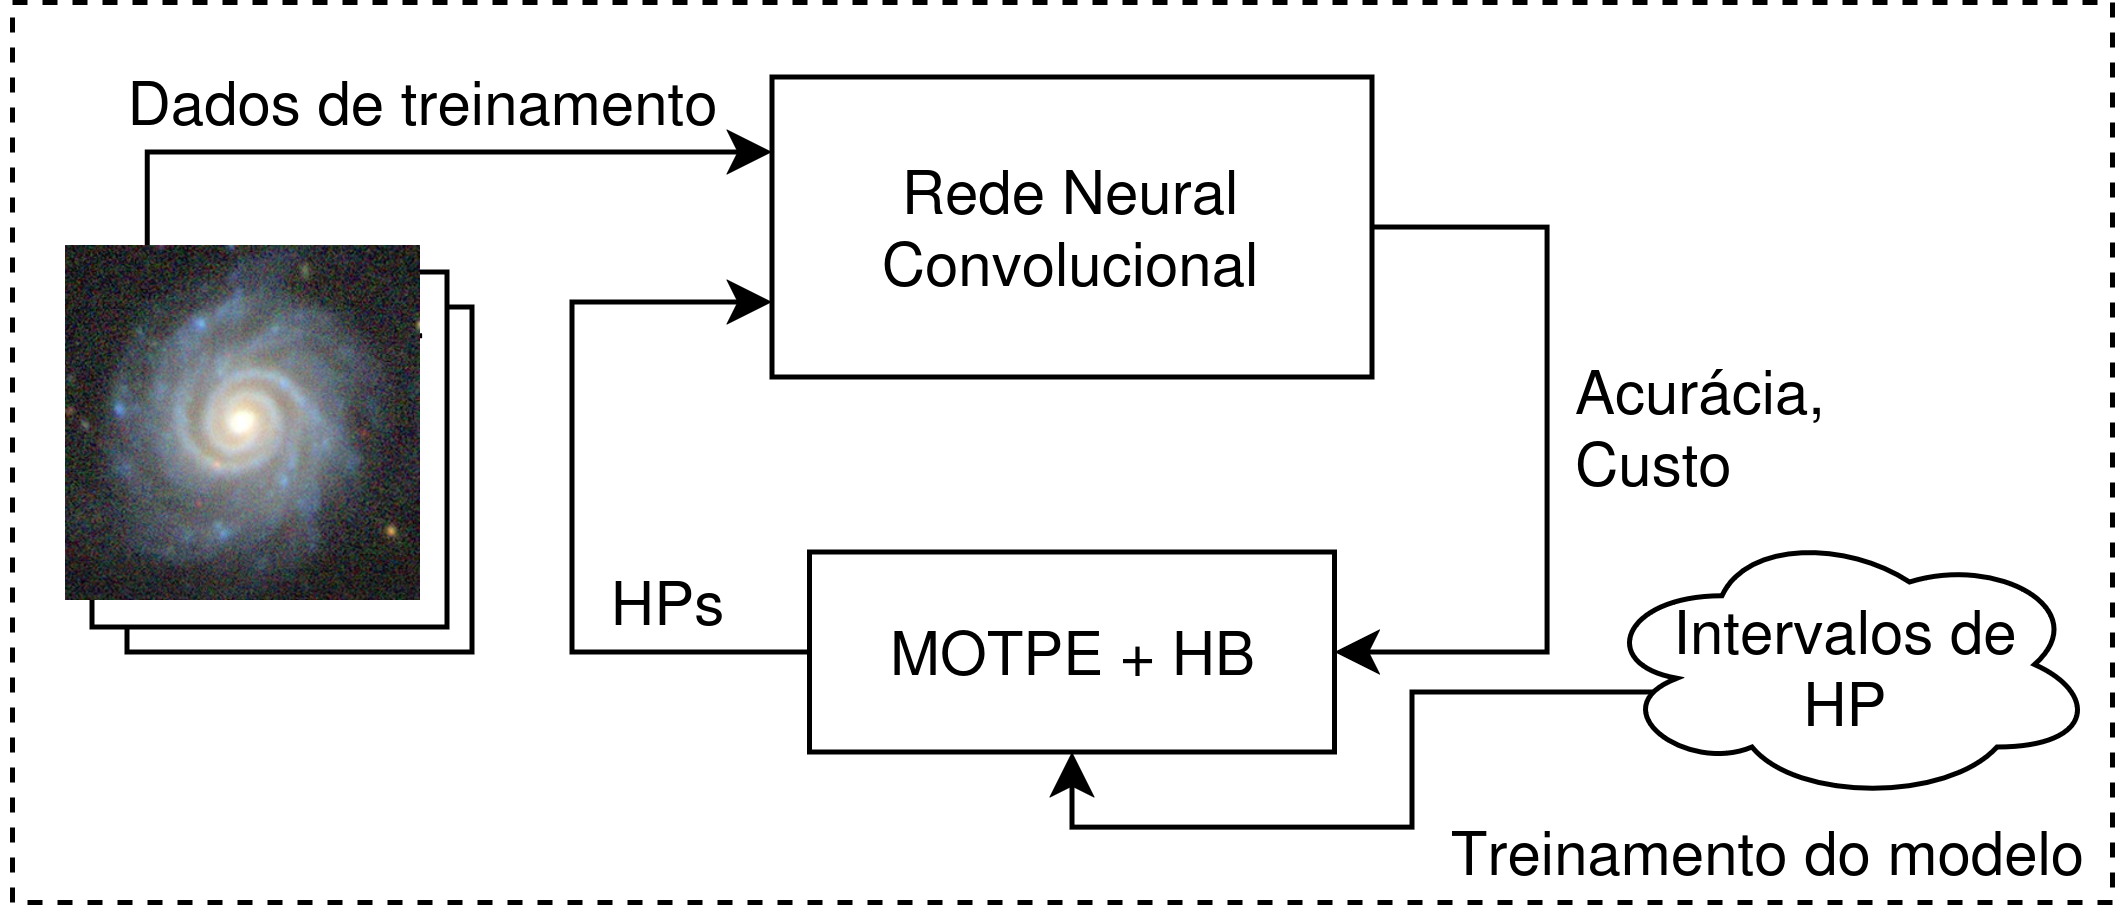
\includegraphics[width=\linewidth]{figures/treinamento.png}
\end{figure}

O treinamento com AutoML utilizando o MOTPE envolve diversas etapas estruturadas, desde a configuração inicial do espaço de busca dos hiperparâmetros até a avaliação iterativa dos modelos. A seguir, descrevem-se as principais etapas do processo:

\begin{enumerate}
  \item \textbf{Definição do Espaço de Busca dos Hiperparâmetros:}
        Inicialmente, define-se um espaço de busca para os hiperparâmetros do modelo, que pode incluir a taxa de aprendizado, número de camadas, número de neurônios por camada, taxas de dropout, tipos de ativação, otimizadores, entre outros. Para cada hiperparâmetro, especificam-se limites, distribuições ou valores discretos que serão explorados pelo algoritmo.

  \item \textbf{Criação da Função de Objetivo:}
        A função de objetivo é o núcleo do processo de otimização. Ela recebe uma configuração de hiperparâmetros como entrada, treina e avalia o modelo utilizando essa configuração, e retorna uma ou mais métricas de desempenho que serão otimizadas. No caso do MOTPE, que é multiobjetivo, é possível considerar métricas conflitantes, como minimizar o erro de validação enquanto reduz o tempo de treinamento.

  \item \textbf{Treinamento Iterativo com Amostragem Bayesiana:}
        O MOTPE utiliza um modelo probabilístico para guiar a busca por configurações promissoras. Ele avalia iterativamente as combinações de hiperparâmetros, ajustando o modelo probabilístico com base nos resultados obtidos em iterações anteriores. Isso permite uma exploração mais eficiente do espaço de busca, concentrando-se em áreas com maior probabilidade de melhorar o desempenho.

  \item \textbf{Validação e Regularização:}
        Cada configuração de hiperparâmetros é validada em um conjunto de validação separado para garantir que o modelo não esteja superajustando os dados de treinamento. Além disso, o uso de técnicas como early stopping e regularização (L2 ou dropout) é integrado ao treinamento para evitar overfitting.

  \item \textbf{Seleção do Melhor Modelo:}
        Após um número predefinido de iterações ou ao atingir um critério de parada, o AutoML seleciona a configuração de hiperparâmetros que apresenta o melhor desempenho médio em relação às métricas otimizadas. No caso de otimização multiobjetivo, a solução é escolhida com base no conceito de fronteira de Pareto.
\end{enumerate}

A Tabela \ref{tab:hps} sumariza os hiperparâmetros otimizados pelo MOTPE. Nela são mostrados os intervalos de busca para cada hiperparâmetro, bem como a distribuição utilizada para cada um deles.


\begin{table}[!ht]
  \centering
  \caption{Intervalos de busca dos hiperparâmetros otimizados com o MOTPE}
  \label{tab:hps}
  \begin{tabular}{lll}
    \toprule
    Hiperparâmetro            & Distribuição     & Intervalo de Busca              \\
    \midrule
    Arquitetura               & Categórica       & \{VGG, IRV2, EffNet, DenseNet\} \\
    Taxa de aprendizado       & Log-Uniforme     & $[10^{-5}, 10^{-1}]$            \\
    Número de camadas ocultas & Int-Uniforme     & $[0, 5]$                        \\
    Neurônios por camada      & Int-Uniforme     & $[32, 512]$                     \\
    Taxa de dropout           & Uniforme         & $[0.1, 0.5]$                    \\
    Otimizador                & Categórica       & \{Adam, NAdam, SGD, RMSprop\}   \\
    Batch size                & Int-Log-Uniforme & $[16, 256]$                     \\
    Peso da regularização L2  & Log-Uniforme     & $[10^{-5}, 10^{-2}]$            \\
    Função de ativação        & Categórica       & \{ReLU, Leaky ReLU, ELU\}       \\
    \bottomrule
  \end{tabular}
\end{table}




\subsection{Métricas de Avaliação da Predição dos Votos}
\label{sec:metricas-votos}

As métricas aqui utilizadas baseiam-se no erro ou acerto na associação dos objetos às classes pelo modelo. Para relacionar a probabilidade calculada pelo modelo à classe, é definido um limiar de discriminação, que é a probabilidade mínima para que um exemplar pertença à uma classe. Para o cálculo das métricas, foi considerado um de limiar de 0.5.

\subsubsection{Matriz de Confusão}
\label{sec:metricas-confusao}

A matriz de confusão consiste em um modelo tabular que cruza métricas de predição e referência, sendo comumente usada para avaliar a qualidade preditiva de modelos de aprendizagem de máquina. A Tabela \ref{tab:cm} mostra um esquema desta matriz para o caso de classificação binária (apenas duas classes). A análise para mais classes pode ser feita isolando uma classe positiva por vez e reduzindo o problema a multiplas classificações binárias.

\begin{table}[!ht]
  \centering
  \caption{Estrutura da matriz de confusão para classificação binária}
  \label{tab:cm}
  \begin{tabular}{lll}
    \toprule
    {}                          & \multicolumn{2}{c}{Predição}                            \\
    \midrule
    \multirow{2}{*}{Verdadeiro} & Verdadeiro Positivo (VP)     & Falso Negativo (FN)      \\
    {}                          & Falso Positivo (FP)          & Verdadeiro Negativo (VN) \\
    \bottomrule
  \end{tabular}
\end{table}

A seguir, são definidas cada uma das métricas usadas para montar a matriz de confusão.

\begin{itemize}
  \item Verdadeiro Positivo (VP): O modelo prevê uma instância verdadeira corretamente
  \item Verdadeiro Negativo (VN): O modelo prevê uma instância negativa corretamente
  \item Falso Positivo (FP): O modelo prevê uma instância positiva, mas, na verdade, é negativa. Este é o erro tipo I, que consiste em rejeitar a hipótese nula quando ela é verdadeira.
  \item Falso Negativo (FN): O modelo prevê uma instância negativa, mas, na verdade, é positiva. Este é o erro tipo II, em estatística, que consiste na falha em rejeitar a hipótese nula quando ela é falsa.
\end{itemize}



\subsubsection{Acurácia}
\label{sec:metricas-acc}

A acurácia é uma métrica que mede a proporção de predições corretas em relação ao total de instâncias avaliadas. Ela é definida como indicado na eq. \ref{eq:acc}.

\begin{equation}\label{eq:acc}
  \text{Acurácia} = \frac{\text{VP} + \text{VN}}{\text{VP} + \text{VN} + \text{FP} + \text{FN}}
\end{equation}



\subsubsection{Precisão}
\label{sec:metricas-precisao}

A precisão avalia a proporção de exemplos classificados como positivos que são realmente positivos, conforme a eq. \eqref{eq:precisao}, sendo particularmente importante em cenários onde o custo de falsos positivos é alto.

\begin{equation}\label{eq:precisao}
  \text{Precisão} = \frac{\text{VP}}{\text{VP} + \text{FP}}.
\end{equation}




\subsubsection{Revocação}
\label{sec:metricas-revocacao}

A revocação, também conhecida como sensibilidade ou taxa de verdadeiros positivos, mede a capacidade do modelo de identificar corretamente os exemplos positivos, conforme a eq. \eqref{eq:recall}, sendo principalmente útil em contextos onde a identificação de todos os exemplos positivos é crucial

\begin{equation}\label{eq:recall}
  \text{Revocação} = \frac{\text{VP}}{\text{VP} + \text{FN}}.
\end{equation}




\subsubsection{F1-Score}
\label{sec:metricas-f1}

O F1-score é a média harmônica entre precisão e revocação, sendo usado como uma métrica de equilíbrio entre essas duas dimensões, conforme a eq. \eqref{eq:f1}. Esta métrica é útil quando há uma compensação entre precisão e revocação, como em cenários com classes desbalanceadas, pois fornece uma medida única que leva em conta ambos os aspectos. Valores de \( F1 \) próximos de 1 indicam que o modelo apresenta um bom equilíbrio entre os dois fatores.

\begin{equation}\label{eq:f1}
  F1 = 2 \cdot \frac{\text{Precisão} \cdot \text{Revocação}}{\text{Precisão} + \text{Revocação}}
\end{equation}






\subsection{Métricas de Avaliação da Similaridade}
\label{sec:metricas-sim}

A recuperação de imagens baseada em embeddings gerados por modelos de aprendizado de máquina envolve a comparação de vetores em um espaço latente para determinar a semelhança ou dissimilaridade entre as representações das imagens. Para isso, são amplamente utilizadas métricas de distância ou similaridade, como similaridade do cosseno (Seção \ref{sec:metricas-cos}), produto interno (Seção \ref{sec:metricas-dot}), distância L1 (Seção \ref{sec:metricas-l1}) e distância L2 (Seção \ref{sec:metricas-l2}). Essas métricas capturam diferentes aspectos das relações entre os embeddings e são escolhidas com base nas características do espaço latente e nos objetivos do sistema. Ademais, nessa Seção, também é definida a métrica que quantifica a capacidade preditiva da tarefa de recuperação por similaridade visual na Seção \ref{sec:metricas-map}.


\subsubsection{Distância do Cosseno}
\label{sec:metricas-cos}

A similaridade do cosseno mede o ângulo entre dois vetores no espaço vetorial, desconsiderando suas magnitudes. Ela é amplamente usada em tarefas de recuperação de imagens e processamento de linguagem natural, pois é invariável à escala dos vetores, o que é útil em embeddings que capturam informações relativas às direções no espaço latente.

Formalmente, ela é definida pela eq. \eqref{eq:cos}, onde \( \mathbf{u} \cdot \mathbf{v} \) é o produto interno dos vetores \( \mathbf{u} \) e \( \mathbf{v} \), e \( \|\mathbf{u}\| \) e \( \|\mathbf{v}\| \) são suas normas. Valores de $\cos(\theta)$ variam entre -1 e 1, onde 1 indica vetores perfeitamente alinhados (paralelos), -1 indica vetores opostos, e 0 indica vetores ortogonais. Já a similaridade do cosseno é mais parecida com outras métricas de distância, pois parte do princípio que coisas próximas possuem valores de distância pequenos, variando de 0 a 2. Quanto mais próximo de zero, mais similar.

\begin{equation}\label{eq:cos}
  \text{Similaridade do Cosseno} = 1-\cos(\theta) = 1-\frac{\mathbf{u} \cdot \mathbf{v}}{\|\mathbf{u}\| \|\mathbf{v}\|}
\end{equation}



\subsubsection{Produto Interno}
\label{sec:metricas-dot}

O produto interno é uma métrica simples que mede a projeção de um vetor sobre outro, conforme a eq. \eqref{eq:dot}, onde \( u_i \) e \( v_i \) são as componentes correspondentes dos vetores \( \mathbf{u} \) e \( \mathbf{v} \). Diferentemente da similaridade do cosseno, o produto interno considera tanto a direção quanto a magnitude dos vetores, o que pode ser útil em espaços latentes onde a magnitude dos embeddings também carrega informações relevantes.

\begin{equation}\label{eq:dot}
  \text{Produto Interno} = \mathbf{u} \cdot \mathbf{v} = \sum_{i=1}^n u_i v_i
\end{equation}



\subsubsection{Distância L1}
\label{sec:metricas-l1}
A distância L1, também conhecida como distância de Manhattan, mede a soma das diferenças absolutas entre as componentes correspondentes de dois vetores. Ela é expressa na eq. \eqref{eq:l1}.

Essa métrica é útil em espaços onde as dimensões são interpretadas como contribuições independentes, e variações locais são importantes. A distância L1 tende a ser mais robusta a outliers do que a distância L2, pois considera contribuições lineares de cada dimensão sem elevar as diferenças ao quadrado.

\begin{equation}\label{eq:l1}
  \text{Distância L1} = \|\mathbf{u} - \mathbf{v}\|_1 = \sum_{i=1}^n |u_i - v_i|
\end{equation}


\subsubsection{Distância L2}
\label{sec:metricas-l2}
A distância L2, ou distância Euclidiana, é a métrica mais comum para medir a similaridade entre vetores. Ela calcula a raiz quadrada da soma dos quadrados das diferenças entre as componentes correspondentes dos vetores, conforme a eq. \eqref{eq:l2}.

Esta métrica é amplamente utilizada devido à sua interpretação geométrica intuitiva como a distância direta entre dois pontos em um espaço multidimensional. No entanto, ela é sensível a outliers, pois penaliza diferenças grandes mais severamente do que a distância L1.

\begin{equation}\label{eq:l2}
  \text{Distância L2} = \|\mathbf{u} - \mathbf{v}\|_2 = \sqrt{\sum_{i=1}^n (u_i - v_i)^2}
\end{equation}




\subsubsection{Métrica de Desempenho da Busca}
\label{sec:metricas-map}
A métrica mAP (mean Average Precision) é amplamente utilizada para avaliar o desempenho de sistemas de recuperação de informações, incluindo a recuperação de imagens baseada em embeddings gerados por modelos de aprendizado de máquina. Essa métrica combina precisão e revocação em um único valor, fornecendo uma medida robusta da capacidade de um modelo em recuperar itens relevantes em tarefas onde a ordenação dos resultados importa.

O cálculo do mAP começa pela definição da \emph{Average Precision} (AP), que mede a precisão média em diferentes níveis de revocação para um conjunto de resultados ordenados. Em um cenário típico de recuperação, para cada consulta, o sistema retorna uma lista ordenada de itens, e o objetivo é avaliar como os itens relevantes estão distribuídos ao longo dessa lista. Dessa forma, para uma consulta \( q \), a AP é definida pela eq. \eqref{eq:ap}, onde \( N \) é o número total de itens retornados; \( P(k) \) é a precisão até a posição \( k \) na lista de resultados; e \( rel(k) \) é uma função indicadora que vale 1 se o item na posição \( k \) for relevante e 0 caso contrário.

\begin{equation}\label{eq:ap}
  AP(q) = \frac{\sum_{k=1}^N P(k) \cdot rel(k)}{\text{Total de itens relevantes}}
\end{equation}

Intuitivamente, a AP calcula a média das precisões em cada ponto onde um item relevante é encontrado, ponderando pela relevância. Isso recompensa sistemas que colocam itens relevantes nas primeiras posições, refletindo a importância da ordenação.

A métrica mAP é obtida como a média da AP sobre todas as consultas \( Q \), conforme a eq. \eqref{eq:map}, onde \( |Q| \) é o número total de consultas. Esse valor sintetiza o desempenho global do sistema, considerando tanto a qualidade das predições individuais quanto a consistência do modelo em diferentes consultas.

\begin{equation}\label{eq:map}
  mAP = \frac{1}{|Q|} \sum_{q \in Q} AP(q)
\end{equation}

O mAP é mais informativo que métricas como acurácia ou precisão isolada, pois considera explicitamente a ordenação dos resultados e é adequado para sistemas de recuperação onde o número de itens relevantes por consulta pode variar. Além disso, o mAP não é influenciado por classes desbalanceadas, pois avalia separadamente a qualidade da recuperação para cada consulta.





\section{Sistema de Informação}
\label{sec:si}


% \begin{figure}[!ht]
%   \caption{Componentes do Sistema de Informação}
%   \label{fig:flow-aquisicao}
%   \begin{center}
%     \smartdiagramset{set color list={orange!60,green!50!lime!60,
%           blue!50!cyan!70!white},
%       % planet color=orange!60,
%       planet size=2.6cm,
%       planet text width=2.6cm,
%       distance planet-satellite=4.0cm,
%       satellite size=3cm,
%       satellite text width=3cm,
%       % uniform connection color=true
%     }
%     \smartdiagram[connected constellation diagram]{
%       Sistema de\\Informação,Base de Dados\\(Seção \ref{sec:si-db}),FrontEnd\\(Seção \ref{sec:si-frontend}),Backend\\(Seção \ref{sec:si-backend})
%     }
%   \end{center}
% \end{figure}
Nesta seção, será descrito desenvolvimento do sistema de informação, esboçado na Fig. \ref{fig:si}, composto por um banco de dados (Seção \ref{sec:si-db}), um backend (Seção \ref{sec:si-backend}) e um frontend (Seção \ref{sec:si-frontend}), que, juntos, são responsáveis pelo armazenamento, manipulação e recuperação dos dados.

\begin{figure}[!ht]
  \centering
  \caption{Diagrama do Sistema de Informação}
  \label{fig:si}
  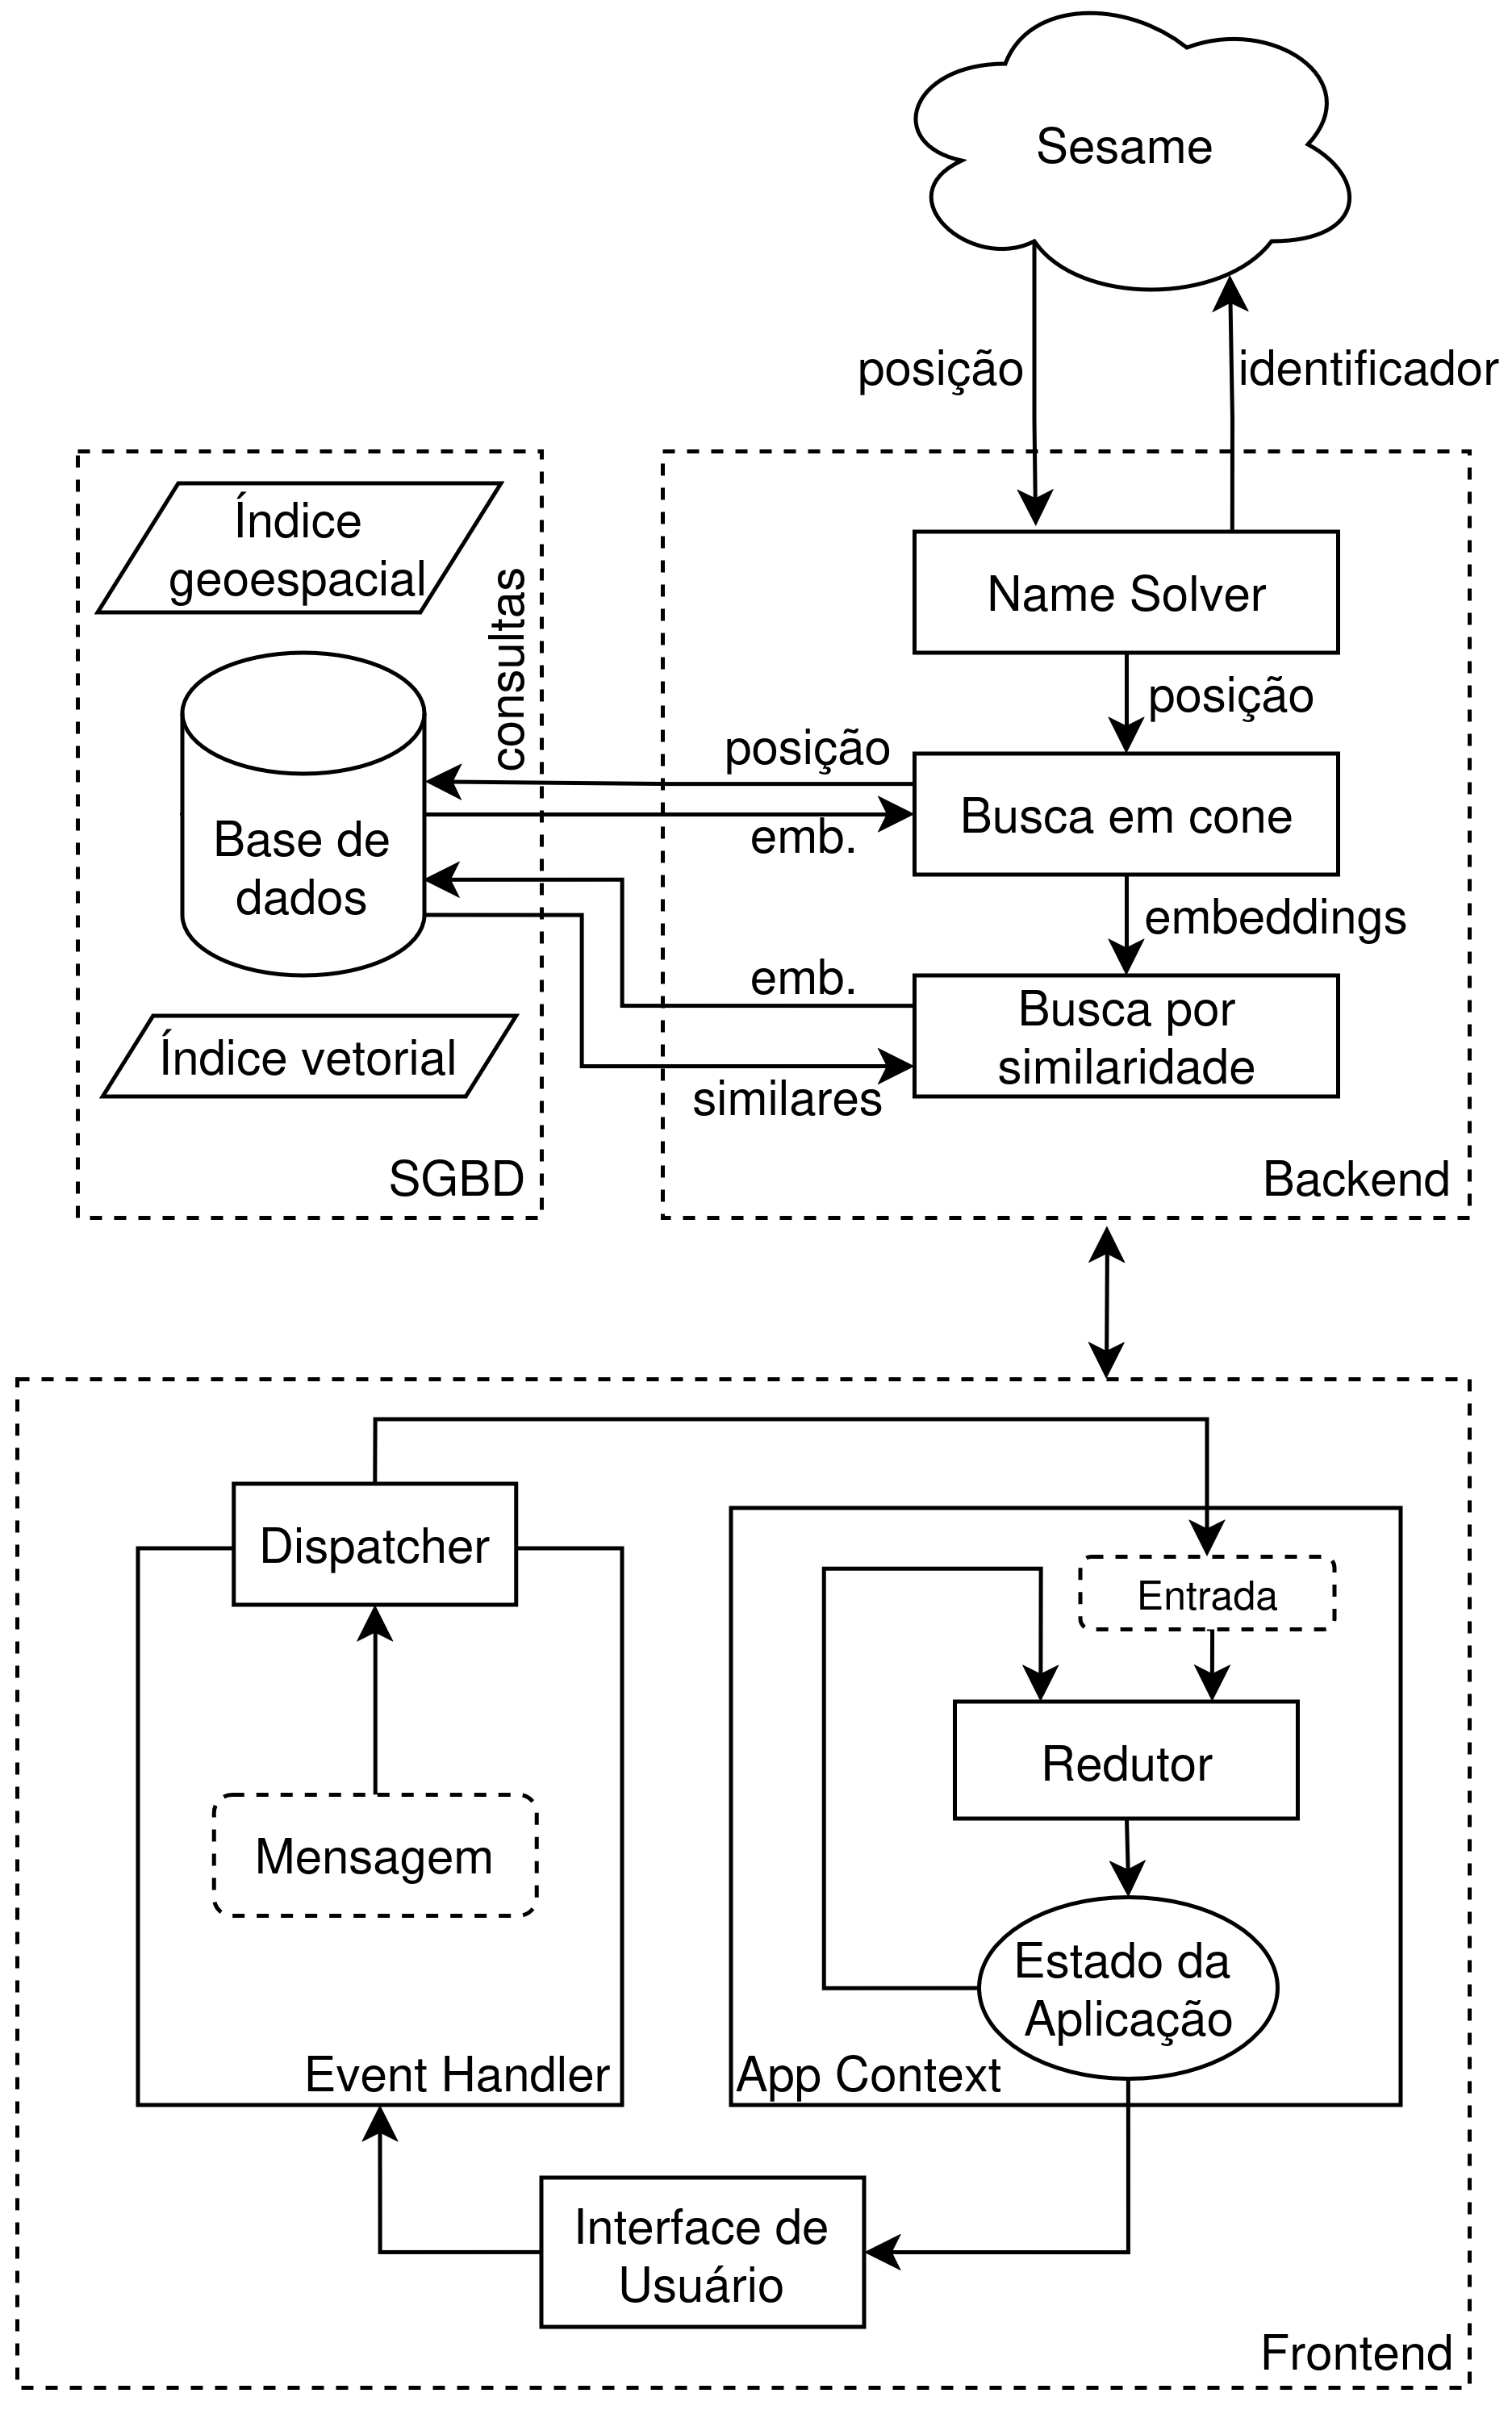
\includegraphics[width=0.75\linewidth]{figures/si.png}
\end{figure}


% \begin{figure}[!ht]
%   \centering
%   \caption{Fluxograma do desenvolvimento do sistema de informação}
%   \label{fig:flow-aquisicao}
%   \simpleflowdiagram{0.5}{
%     Base de Dados (Seção \ref{sec:si-db}),
%     Backend (Seção \ref{sec:si-backend}),
%     Frontend (Seção \ref{sec:si-frontend}),
%     Implantação (Seção \ref{sec:si-implantacao})
%   }
% \end{figure}



\subsection{Base de Dados}
\label{sec:si-db}

A base de dados desempenha um papel fundamental no sistema inteligente desenvolvido, pois ela tem a função de armazenar as representações visuais, geradas a partir do modelo do aprendizagem profunda (Seção \ref{sec:modelo}) e delimitadas pelo conjunto de inferência (Seção \ref{sec:aquisicao-inferencia}), com o propósito de viabilizar a busca rápida no céu por similaridade visual em uma grande área do céu. Esta funcionalidade foi especificada durante a concepção do projeto como o  requisito funcional de armazenamento e recuperação de representações visuais (Seção \ref{sec:req-db}). A seguir, são discutidas as tecnologias  (Seção \ref{sec:si-tecnologias}), o modelo de dados (Seção \ref{sec:si-datamodel}) e as otimizações (Seções \ref{sec:si-coords-index} e \ref{sec:si-vec-index}) utilizadas do desenvolvimento da base de dados.

% No Sistema Inteligente proposto, a base de dados tem a função de armazenar as representações visuais, geradas a partir do modelo do aprendizagem profunda (Seção \ref{sec:modelo}) e delimitadas pelo conjunto de inferência (Seção \ref{sec:aquisicao-inferencia}), com o propósito de viabilizar a busca rápida no céu por similaridade visual em uma grande área do céu.



\subsubsection{Tecnologias Utilizadas}
\label{sec:si-tecnologias}

Uma parte fundamental no projeto de uma base de dados é a escolha do Sistema Gerenciador de Banco de Dados (SGBD), essa escolha está fortemente relacionada com o tipo de dado a ser armazenado e os tipos de buscas a serem realizadas. Nesse sentido, para atender os requisitos da aplicação desenvolvida, as especificações do SGBD são listadas a seguir.

\begin{itemize}
  \item \textbf{Armazenamento de vetores:} as características visuais extraídas pelo modelo de aprendizagem profunda (Seção \ref{sec:modelo}) são representadas na forma de vetores. Logo, é essencial que o SGBD  consiga manusear esse tipo de dado;
  \item \textbf{Busca eficiente de vetores:} a recuperação de objetos similares é a busca por obejtos com menor distância do vetor de referêcia. Nesse sentido, o SGBD precisa realizar operações com distância de vetores além de ter um mecanismo de indexação que otimize a busca por distância;
  \item \textbf{Busca por posição:} além das representações visuais, a base de dados deve armazenar metadados dos objetos, como a posição. A busca por posição é fundamental para integrar o sistema como outros serviços web astronômicos, como Sesame, Simbad e Vizier, pois ela permite correlacionar informações de um mesmo objeto proveniente de fontes diferentes.
\end{itemize}

Com base nas especificações apresentadas e levando em consideração as tecnologias do estado-da-arte para a tarefa desenvolvida \cite{pan2024}, o PostgreSQL\footnote{\url{https://postgresql.org}} foi ecolhido como SGDB, pois sua flexibilidade e extensibilidade permitem as funcionalidades de busca por posição e vetorial, discutidas nas Seções \ref{sec:si-coords-index} e \ref{sec:si-vec-index}, respectivamente.


\subsubsection{Modelo de Dados}
\label{sec:si-datamodel}

A definição de um modelo de dados eficiente é fundamental para a integração das diversas partes do sistema. A Fig. \ref{fig:db} mostra o diagrama entidade-relacionamento da base de dados projetada para o armazenamento e a recuperação dos objetos por similaridade visual.

\begin{figure}[!ht]
  \centering
  \caption{Diagrama entidade-relacionamento da base de dados}
  \label{fig:db}
  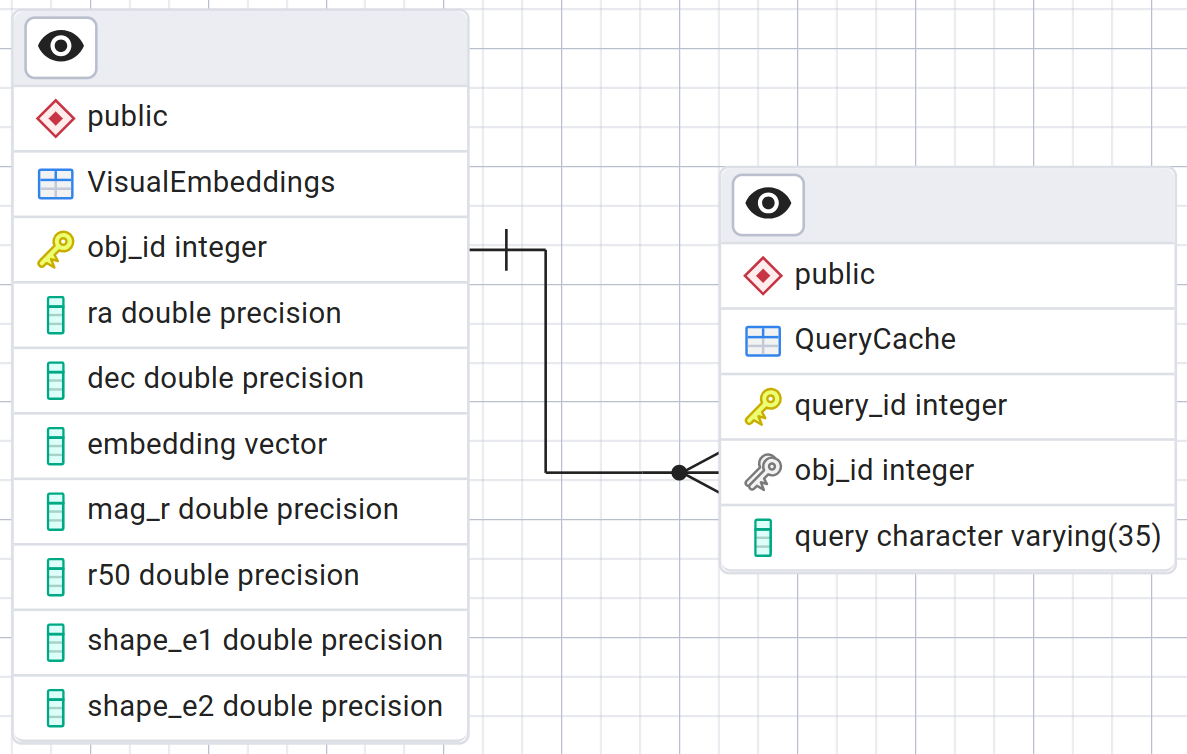
\includegraphics[width=\linewidth]{figures/database.png}
  \legend{O diagrama entidade-relacionamo mostra duas tabelas: \texttt{VisualEmbeddings} (esquerda) e \texttt{QueryCache} (direita). A primeira armazena as representações visuais e algumas propriedades físicas de todas as galáxias do conjunto de inferência (Seção \ref{sec:aquisicao-inferencia}). Já a segunda é um cache que associa um termo de busca à chave primária da tabela anterior, tendo a função de evitar requisição ao sistema Sesame e a correlação por coordenadas.}
\end{figure}


As Tabelas \ref{tab:VisualEmbeddings} e \ref{tab:QueryCache} informam o tipo de dado e uma breve descrição de cada coluna das tabelas mostradas na Fig. \ref{fig:db}.

A indexação de colunas é um mecanismo fundamental de otimização de consultas em bases de dados relacionais, representando os dados por uma estrutura de dados auxiliar, projetada para garantir mais desempenho em tipos específicos de problemas. Na sequência, são mostradas as técnicas de indexação para as colunas \texttt{ra} e \texttt{dec} (Seção \ref{sec:si-coords-index}) e para a coluna \texttt{embedding} (Seção \ref{sec:si-vec-index}).

\begin{table}[!ht]
  \centering
  \caption{Descrição da tabela VisualEmbeddings}
  \label{tab:VisualEmbeddings}
  \begin{tabular}{rlp{.6\linewidth}}
    \toprule
    Coluna    & Tipo           & Descrição                                                                     \\
    \midrule
    obj\_id   & inteiro        & Chave primária do objeto                                                      \\
    ra        & precisão dupla & Ascenção Reta do obejeto (Seção \ref{sec:sistema-coordenadas})                \\
    dec       & precisão dupla & Declinação do obejeto (Seção \ref{sec:sistema-coordenadas})                   \\
    embedding & vetor          & Vetor de representações visuais                                               \\
    mag\_r    & precisão dupla & Magnitude do objeto (Seção \ref{sec:magnitude})                               \\
    shape\_e1 & precisão dupla & Componente real da elipticidade complexa (Seção \ref{sec:elipticidade})       \\
    shape\_e2 & precisão dupla & Componente imaginária da elipticidade complexa (Seção \ref{sec:elipticidade}) \\
    % fov       & precisão dupla & Campo de visão angular ideal para o objeto, em arcsec (Seção \ref{sec:aquisicao-fov})     \\
    \bottomrule
  \end{tabular}
\end{table}


\begin{table}[!ht]
  \centering
  \caption{Descrição da tabela QueryCache}
  \label{tab:QueryCache}
  \begin{tabular}{rlp{.6\linewidth}}
    \toprule
    Coluna    & Tipo    & Descrição                                                                                                     \\
    \midrule
    query\_id & inteiro & Chave primária                                                                                                \\
    obj\_id   & inteiro & Chave estrangeira referenciando a coluna obj\_id da tabela VisualEmbeddings (Tab. \ref{tab:VisualEmbeddings}) \\
    query     & string  & Termo de busca utilzado para fazer a consulta                                                                 \\
    \bottomrule
  \end{tabular}
\end{table}



\subsubsection{Armazenamento e Indexação das Coordenadas}
\label{sec:si-coords-index}

A indexação das coordenadas, definidas pelas colunas \texttt{ra} e \texttt{dec}, utiliza o mecanismo Quad Tree Cube\footnote{\url{https://github.com/segasai/q3c}} (Q3C; \citealp{q3c}), que é uma técnica utilizada na astronomia para otimizar o armazenamento e a recuperação de dados espaciais em bancos de dados de grandes levantamentos astronômicos. Esse mecanismo foi desenvolvido para lidar com a quantidade massiva de dados gerada por observatórios modernos, que capturam informações sobre bilhões de objetos celestes, incluindo sua posição, brilho e outras características. A principal função do Q3C é permitir consultas eficientes em catálogos astronômicos, possibilitando a localização rápida de objetos com base em suas coordenadas celestes (Seção \ref{sec:sistema-coordenadas}).

O Q3C utiliza uma estrutura baseada em árvore quad (ou quadtree) projetada para dividir iterativamente a superfície da esfera celeste (Seção \ref{sec:sistema-coordenadas}) em regiões menores, como mostra a Fig. \ref{fig:q3c}. Cada região é identificada por um índice (chamado IPIX), o que permite armazenar e acessar informações de localização de forma hierárquica. No Q3C, a superfície esférica é projetada em um cubo e subdividida em quadrantes, o que facilita a representação de posições celestes e otimiza a indexação espacial. Essa estrutura de dados permite que consultas espaciais, como encontrar todos os objetos dentro de um certo raio de um ponto específico, sejam executadas com alta eficiência, reduzindo a necessidade de examinar todas as entradas do catálogo.

\begin{figure}[!ht]
  \centering
  \caption{Segmentação da esfera celeste pelo Q3C}
  \label{fig:q3c}
  \begin{overpic}[width=.32\linewidth]{figures/q3c_1.png}
    \put (0,90) {(a)}
  \end{overpic}\hfill
  \begin{overpic}[width=.32\linewidth]{figures/q3c_2.png}
    \put (0,90) {(b)}
  \end{overpic}\hfill
  \begin{overpic}[width=.32\linewidth]{figures/q3c_3.png}
    \put (0,90) {(c)}
  \end{overpic}
  \legend{Nos painéis (a) e (b), são mostradas segmentações da esfera celeste (Seção \ref{sec:sistema-coordenadas}) pelo Q3C para duas quantidades de bits distintas. Já o painel (c) mostra um exemplo de busca usando o Q3C. Fonte: Compilação das Figs. 1 e 2 de \citeonline{q3c}.}
\end{figure}

A implementação do Q3C aproveita funções de hashing para transformar as coordenadas esféricas em valores que podem ser facilmente indexados. Esse processo de hash mapeia coordenadas (RA, DEC) para uma representação numérica, permitindo uma indexação que é eficiente tanto para operações de busca por proximidade quanto para consultas de intervalo. As consultas são formuladas de maneira que a hierarquia de quadrantes seja explorada, de modo que apenas uma fração dos dados seja analisada para atender à consulta. Além disso, o Q3C pode realizar operações de cruzamento de catálogos, comparando dados de diferentes levantamentos com rapidez.


\subsubsection{Armazenamento e Indexação dos Vetores}
\label{sec:si-vec-index}

Embora o PostgreSQL seja tradicionalmente um banco de dados relacional, sua flexibilidade e extensibilidade permitem a implementação de funcionalidades tipicamente associadas a bancos de dados vetoriais \cite{taipalus2024}, como o armazenamento e a busca eficiente de vetores. Isso é alcançado por meio de extensões, como o pgvector\footnote{\url{https://github.com/pgvector/pgvector}}, que integram capacidades vetoriais ao PostgreSQL. Com essa abordagem, é possível armazenar vetores diretamente em tabelas relacionais e realizar consultas por similaridade, transformando o PostgreSQL em uma solução híbrida que combina recursos relacionais e vetoriais.

O mecanismo de indexação de vetores no pgvector é projetado para otimizar a indexação e busca de embeddings de alta dimensionalidade, especialmente aqueles gerados por modelos de aprendizagem profunda. Tais representações são amplamente utilizadas em aplicações como recuperação de informação, recomendação e classificação de dados, onde é necessário medir similaridade entre itens com base em seus embeddings. O pgvector oferece suporte nativo para armazenar e indexar esses vetores no PostgreSQL, tornando viável a realização de buscas eficientes mesmo em bancos de dados com grandes volumes de dados vetoriais.

O pgvector utiliza o HNSW, uma estrutura de grafos, chamada Hierarchical Navigable Small World Graph (HNSW; \citealp{hnsw}), que facilita a busca aproximada por similaridade. O HNSW é baseado em uma hierarquia de grafos navegáveis, onde cada nó representa um vetor, e conexões entre nós são criadas com base na similaridade vetorial. Esse grafo permite uma navegação eficiente, utilizando uma busca aproximada que, apesar de não garantir a precisão absoluta, oferece um bom equilíbrio entre desempenho e precisão. O HNSW é particularmente eficaz em cenários com alta dimensionalidade, pois reduz o número de cálculos de similaridade necessários para encontrar o vetor mais próximo, sendo capaz de realizar buscas sublineares em grandes volumes de dados. Em termos de aplicação prática, esse método torna viável a busca por similaridade em bancos de dados com milhões de embeddings, permitindo um tempo de resposta mais rápido.



\subsection{Backend}
\label{sec:si-backend}

O backend refere-se à camada responsável pelo processamento lógico, manipulação de dados e comunicação com bancos de dados e serviços externos. Ele opera nos servidores e é invisível ao usuário final, funcionando como a infraestrutura que sustenta e executa as operações solicitadas pelo frontend. O backend normalmente utiliza frameworks e ferramentas para gerenciar APIs, autenticação, controle de acesso e persistência de dados. Sua principal função é garantir que as informações sejam processadas de forma segura, eficiente e escalável, permitindo que a aplicação ofereça funcionalidades dinâmicas aos usuários.


\subsubsection{Tecnologias Utilizadas}
\label{sec:si-back-tech}

O desenvolvimento do backend requer a utilização de tecnologias que garantam desempenho, escalabilidade e flexibilidade. Nesse contexto, a biblioteca Blacksheep\footnote{\url{https://www.neoteroi.dev/blacksheep}}, implementada em Python, oferece uma solução moderna para construir APIs robustas e eficientes. Trata-se de um framework assíncrono que utiliza o modelo de programação baseado em corrotinas do Python, permitindo lidar de maneira eficiente com operações de entrada e saída (E/S) intensivas, como consultas a bancos de dados de grande escala.

A Blacksheep é projetada sobre o motor de eventos do módulo asyncio, proporcionando suporte nativo para o desenvolvimento de APIs RESTful de alta performance. Sua abordagem assíncrona é vantajosa para sistemas que requerem comunicação frequente com bancos de dados, como é o caso deste sistema de recuperação de imagens astronômicas. Além disso, a biblioteca adota um design simples e modular, permitindo personalizar funcionalidades conforme necessário.

Foram utilizados os middlewares e roteamento eficiente da biblioteca Blacksheep, possibilitando a construção de uma API organizada e segura. A biblioteca também integra-se facilmente com o SQLAlchemy, essencial em aplicações astronômicas, que frequentemente demandam operações complexas de busca e agregação de dados.

% Adicionalmente, a Blacksheep oferece suporte a recursos como validação de dados, serialização e uso de controladores baseados em classes, promovendo uma estrutura clara e sustentável para o código. A compatibilidade com tecnologias modernas, como OpenAPI e JSON Schema, facilita a documentação automática da API, melhorando a interoperabilidade e o desenvolvimento colaborativo. Essas vantagens tornam a Blacksheep uma escolha ideal para implementar o backend de um sistema que requer alta responsividade, modularidade e suporte a consultas complexas, como a recuperação de imagens por similaridade visual em astronomia.




\subsubsection{Integrações}
\label{sec:si-back-arch}

O backend é composto por uma API RESTful responsável por implementar a lógica de consulta por similariade e permitir o acesso aos dados pelo frontend. Pensando em aumentar a flexibilidade e a experiência de usuário, o sistema permite que a busca seja feito pelo nome oficial da galáxia, apelido ou coordenada. Para garantir essa funcionalidade, é necessária uma interação com o webserviço astronômico \emph{Sesame Name Solver}\footnote{\url{https://cds.unistra.fr/cgi-bin/Sesame}}, que é utilizado para resolver o termo de busca enviado pelo usuário, convertendo-o em posição angular da galáxia (RA e Dec).

% Buscas por posição e por similaridade são feitas pelo backend para




% \begin{figure}[!ht]
%   \centering
%   \caption{Diagrama da arquitetura do backend}
%   \label{fig:backend}
%   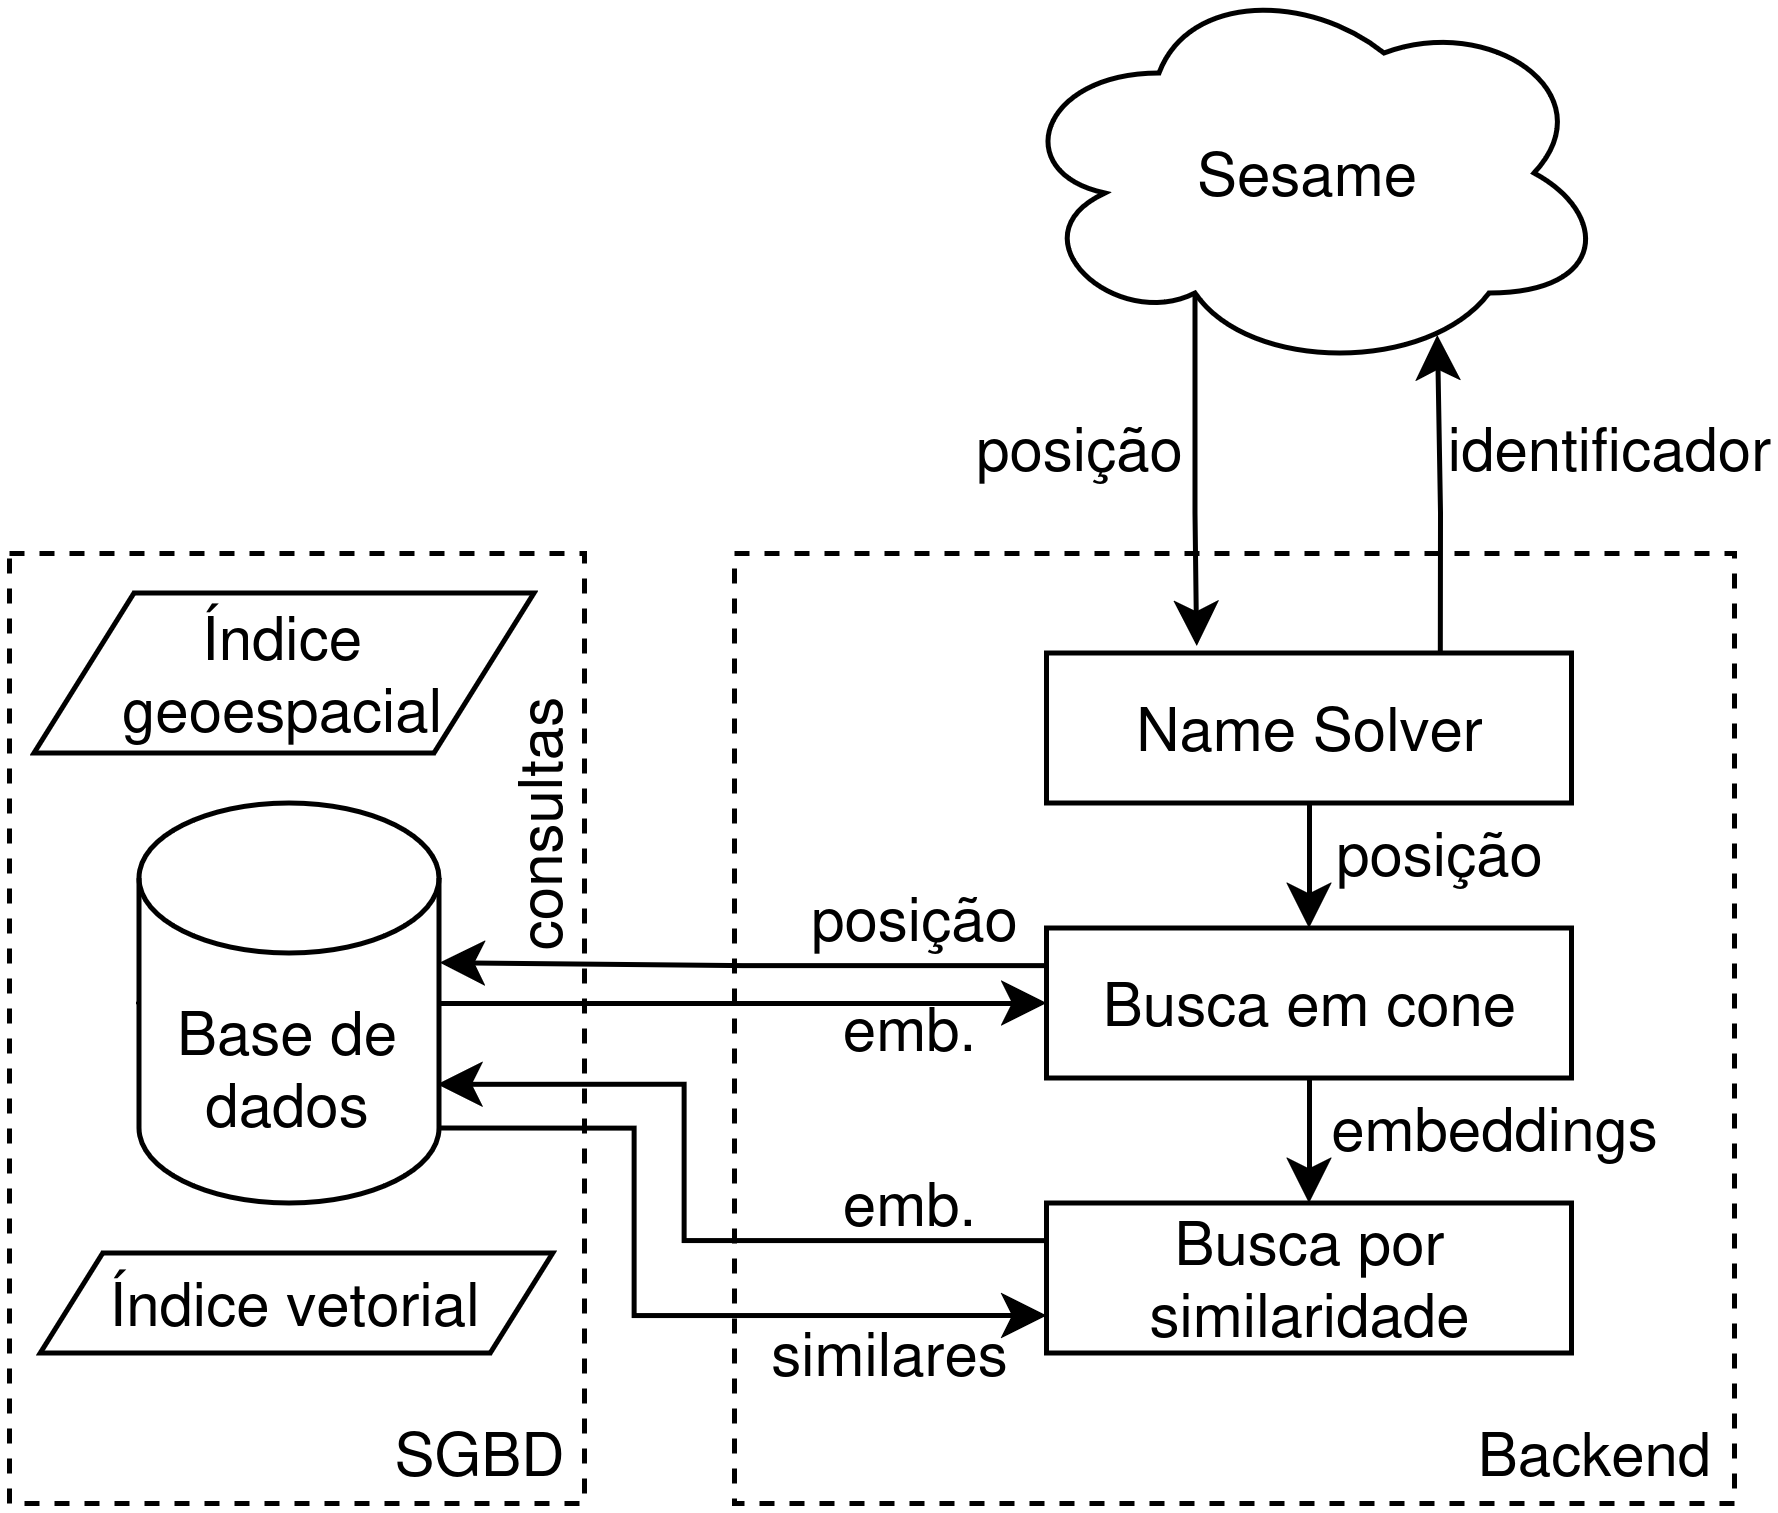
\includegraphics[width=0.8\linewidth]{figures/backend.png}
% \end{figure}




\subsubsection{Procedimento de Busca no Backend}
\label{sec:si-bacak-busca}

A Fig. \ref{fig:seq-back} mostra o diagrama de sequência do procedimento de busca por similaridade visual do ponto de vista do backend. Nela é mostrada as três etapas da busca: a resolução do nome do objeto, transformando-o em coordenadas; a busca por posição no banco de dados para encontrar os embeddings da galáxia buscada e, por fim, a busca por similaridade.

\begin{figure}[!ht]
  \centering
  \caption{Diagrama de sequência da busca no backend}
  \label{fig:seq-back}
  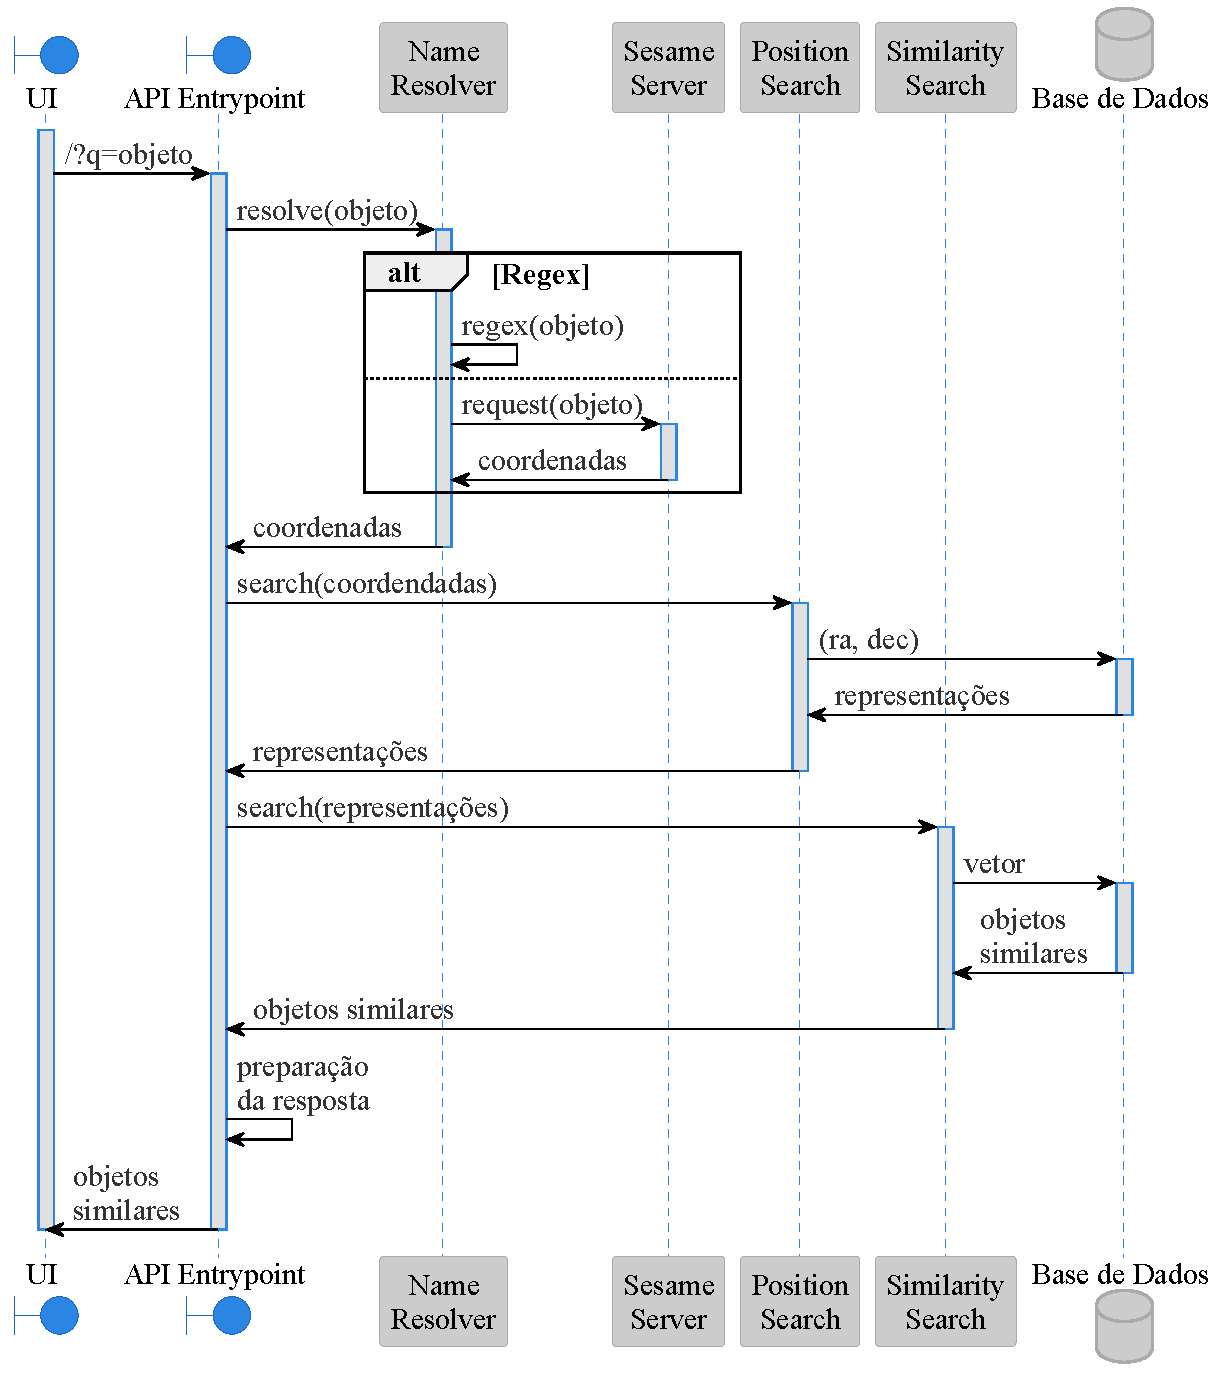
\includegraphics[width=\linewidth]{diagrams/plots/sequence_back.pdf}
  \legend{Primeiramente, o termo de busca é decodificado em coordenadas RA e Dec utilizando o webserviço Sesame. Em seguida, uma busca por posição é feita no banco de dados para obter as representações da galáxia busca. Por fim, é feita uma busca por similaridade para obter as galáxias similares.}
\end{figure}






\subsection{Frontend}
\label{sec:si-frontend}

O frontend refere-se à camada da aplicação interpretada diretamente pelo navegador responsável pela interface visual e interação direta com o usuário. Ele abrange a estrutura, o estilo e o comportamento das páginas ou telas que os usuários visualizam e utilizam. O frontend conecta-se ao back-end por meio de APIs, recebendo e enviando dados para apresentar informações dinâmicas e garantir uma experiência de uso interativa e responsiva.


\subsubsection{Tecnologias Utilizadas}
\label{sec:si-front-tech}

O frontend é a camada da aplicação que é executada no navegador. Ele foi desenvolvido em TypeScript\footnote{\url{https://typescriptlang.org}}, que é uma linguagem de programação de código aberto que expande o JavaScript ao adicionar suporte a tipagem estática e outras funcionalidades avançadas de desenvolvimento. O TypeScript é amplamente utilizado para melhorar a robustez e a escalabilidade do código, permitindo a detecção de erros em tempo de compilação e facilitando a manutenção de projetos complexos. As aplicações feitas nesta linguagem são transpiladas para JavaScript para serem interpretadas pelos navegadores.

O frontend foi desevolvido utilzando o Next.js\footnote{\url{https://nextjs.org}}, que é um framework de desenvolvimento web baseado na biblioteca React que permite a criação de aplicações modernas e escaláveis. A principal ferramenta usada é a geração estática (Static Site Generation, SSG), que permite compilar e distribuir o frontend como uma aplicação completamente independente do backend. Além disso, o Next.js fornece uma estrutura que simplifica o desenvolvimento ao incluir funcionalidades integradas, como roteamento automático baseado em arquivos, suporte a APIs serverless, otimização de desempenho e internacionalização.

A biblioteca React\footnote{\url{https://react.dev}} revolucionou a forma como interfaces de usuário (UI) são projetadas e construídas no desenvolvimento de aplicativos modernos. Baseada no conceito de componentes reutilizáveis, o React permite que desenvolvedores criem aplicações web e móveis de forma declarativa, eficiente e altamente escalável.


\subsubsection{Arquitetura}
\label{sec:si-front-arch}

Um dos principais diferenciais do React é sua abordagem declarativa para o desenvolvimento de UI. Em vez de manipular diretamente o Document Object Model (DOM), os desenvolvedores descrevem como a interface deve se comportar em diferentes estados, e o React cuida de atualizar o DOM de maneira eficiente. Essa abstração é possibilitada pelo Virtual DOM, uma representação leve do DOM real que permite ao React identificar e aplicar somente as alterações necessárias, minimizando a manipulação direta do DOM e melhorando o desempenho de aplicativos, especialmente em sistemas complexos com múltiplos estados dinâmicos.


\begin{figure}[!ht]
  \centering
  \caption{Arquitetura do gerenciamento de estado da interface de usuário}
  \label{fig:arch-front}
  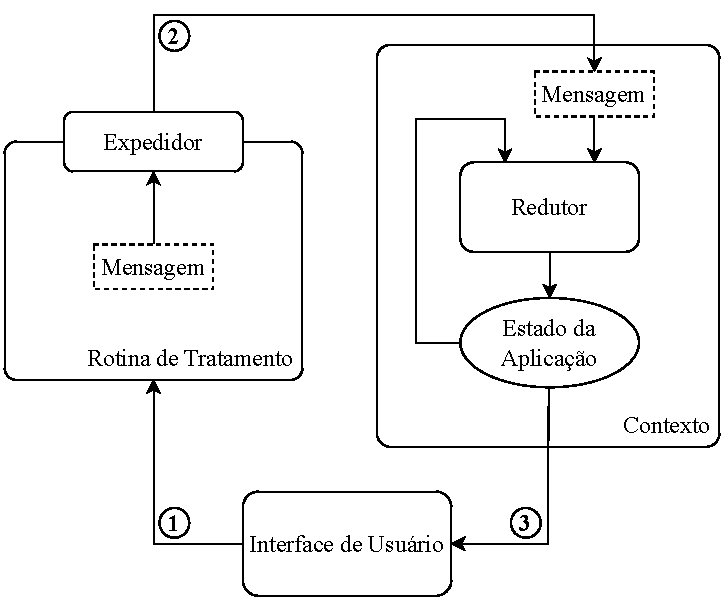
\includegraphics[width=0.8\linewidth]{figures/flow_front.pdf}
\end{figure}

Nessa abordagem declarativa, o gerenciamento de estado da aplicação é o mecanismo mais importante. Este mecanismo pode ser visto como uma máquina de estados finita \cite{formal-methods} que depende do estado atual e uma entrada para produzir o próximo estado, como a máquina \citeonline{mealy}. Este mecanismo é ilustrado no diagrama da Fig. \ref{fig:arch-front} e seus elementos são explicados a seguir.

\begin{enumerate}
  \item O usuário interage com a \emph{Interface do Usuário} (UI), causando um evento, que é enviado para a \emph{Rotina de Tratamento}. Este evento pode ser um clique do mouse, um pressionamento de tecla, uma seleção de arquivo e assim por diante.
  \item A \emph{Rotina de Tratamento} é a função responsável por processar o evento. Como o sistema é desenvolvido usando abordagem declarativa, ao invés de executar alterações diretas na UI, esta função prepara uma mensagem contendo todas as informações necessárias para mudar a aplicação para outro estado e passá-la para o \emph{Expedidor}, responsável por enviar a mensagem para o \emph{Redutor}.
  \item O \emph{Redutor} é a função, chamada pelo \emph{Contexto da Aplicação}, responsável por gerar o próximo estado da aplicação. Esta função recebe o estado atual e a mensagem do \emph{Expedidor} para criar um novo estado. A mutação no \emph{Estado da Aplicação} dispara a atualização da UI, realizada pela biblioteca React. O \emph{Redutor} pode ser visto como a função de transição da Máquina Mealy.
\end{enumerate}


Além disso, a arquitetura baseada em componentes do React é outro ponto crucial para seu sucesso. Aplicações são divididas em partes menores e independentes, chamadas componentes, que encapsulam lógica, estilo e estrutura de forma modular. Esses componentes podem ser reutilizados em diferentes partes de um aplicativo ou até mesmo em projetos distintos, promovendo consistência no design e eficiência no desenvolvimento. Além disso, a reutilização de componentes reduz o tempo necessário para implementar novas funcionalidades e simplifica a manutenção do código, uma característica essencial para projetos modernos, que frequentemente envolvem equipes de desenvolvimento distribuídas e de grande escala.


\subsubsection{Procedimento de Busca no Frontend}
\label{sec:si-front-busca}

A Fig. \ref{fig:seq-front} mostra o diagrama de sequência do procedimento de busca por similaridade visual do ponto de vista do frontend.

\begin{figure}[!ht]
  \centering
  \caption{Diagrama de sequência da busca no frontend}
  \label{fig:seq-front}
  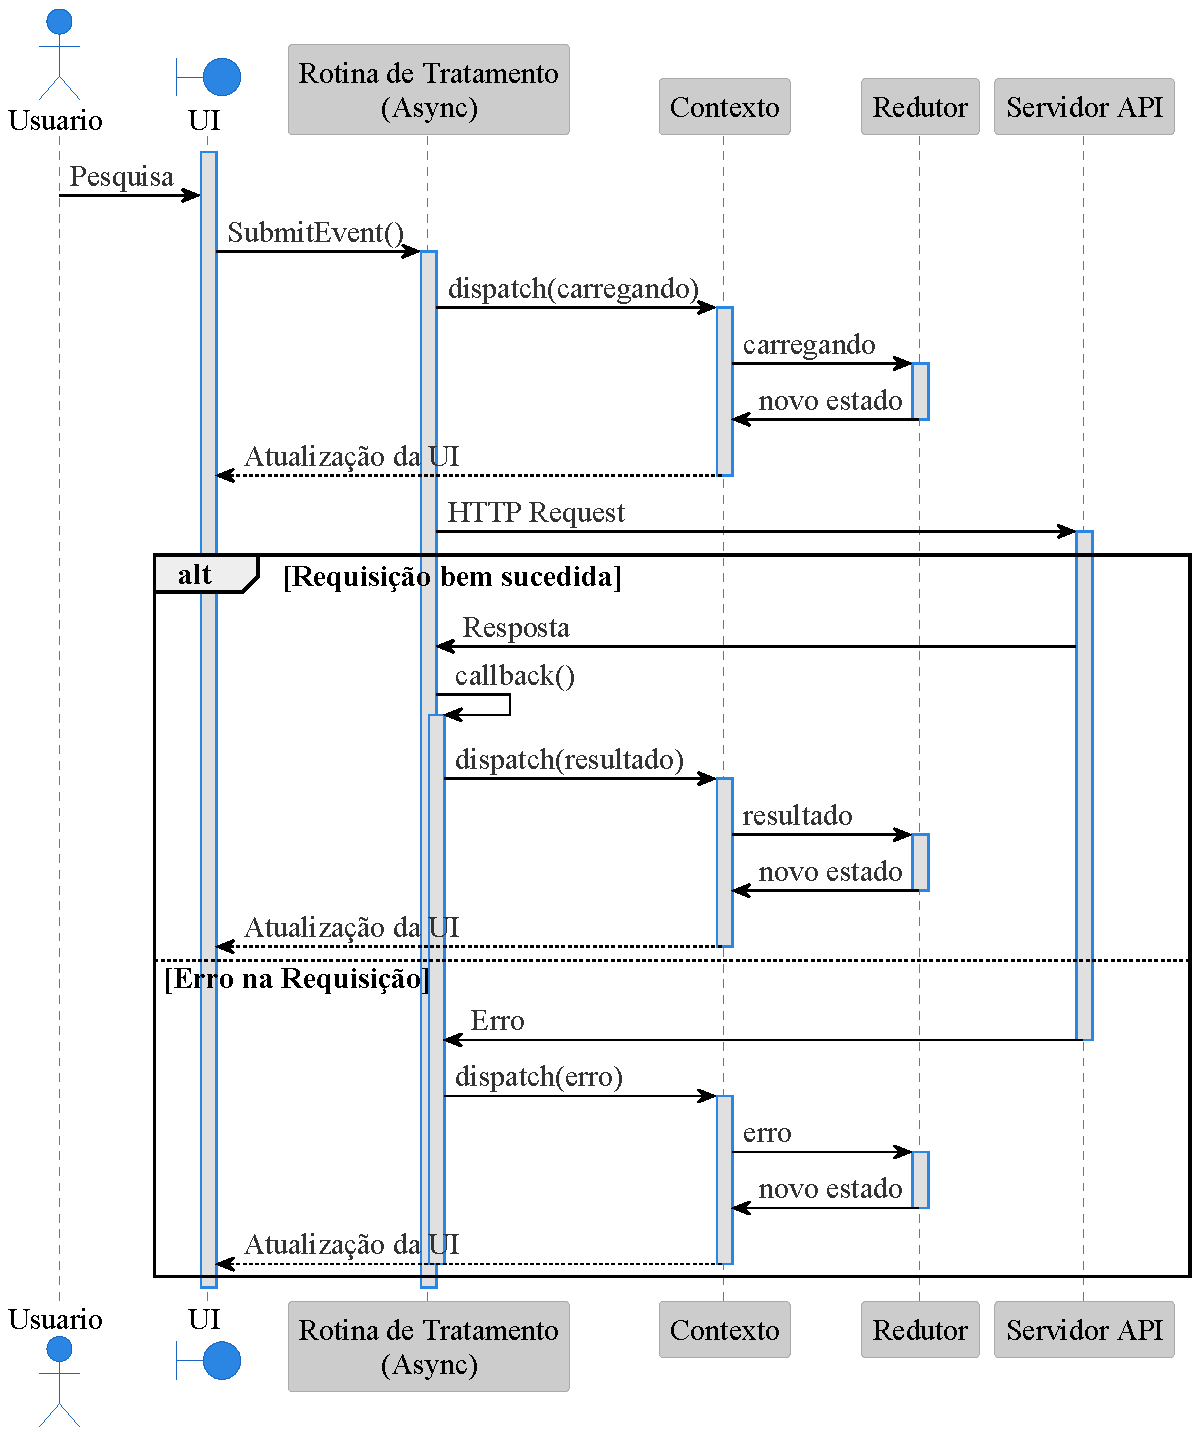
\includegraphics[width=\linewidth]{diagrams/plots/sequence_front.pdf}
  \legend{Ao interagir com a barra de pesquisa, o usuário engatilha um evento, que é interceptado pelo motor de eventos do navegador, que inicializa a rotina de tratamento registrada para o evento. Esta função despacha uma mensagem, ao contexto da aplicação, para mudar o estado da UI para ``carregando'' e, em seguida, faz uma requisição HTTP ao servidor. Ao receber a resposta da API, a função callback é responsável por despachar uma mensagem com os resultados ou com erro, causando uma nova atualização da UI.}
\end{figure}



\subsection{Implementação e Implantação}
\label{sec:si-implantacao}

Nesta seção, são abordadas as técnicas de desenvolvimento e implantação utilizadas para a disponibilização do sistema de informação desenvolvido como uma aplicação web.


\subsubsection{Sistema de Controle de Versão}
\label{sec:si-devops}

O uso combinado do sistema de controle de versão Git e da plataforma GitHub\footnote{\url{https://github.com}} no desenvolvimento de um sistema inteligente para busca de imagens similares em astronomia oferece uma série de vantagens que otimizam a colaboração, a gestão do código e a automação de processos. O Git\footnote{\url{https://git.org}}, sendo um sistema distribuído, permite que os desenvolvedores rastreiem todas as alterações feitas no código-fonte de forma detalhada, possibilitando reverter modificações indesejadas e garantir a integridade do desenvolvimento. Sua estrutura descentralizada assegura que cada colaborador mantenha uma cópia completa do repositório, aumentando a segurança e a resiliência contra falhas.

A integração com o GitHub amplia essas capacidades, oferecendo uma interface intuitiva e funcionalidades adicionais que promovem o trabalho em equipe. A plataforma facilita a criação de ramificações (branches) para desenvolvimento paralelo, revisão de código por meio de pull requests e resolução de conflitos de forma transparente. Tais recursos são fundamentais em projetos de sistemas inteligentes, onde equipes frequentemente trabalham em componentes diferentes, como algoritmos de similaridade, infraestrutura de backend e interfaces gráficas.

Além disso, o GitHub fornece ferramentas de integração contínua (CI) e entrega contínua (CD), permitindo a execução automática de testes, validações e implantações a cada mudança no código. Isso reduz significativamente o risco de erros e acelera o ciclo de desenvolvimento, o que é crucial em projetos que lidam com grandes volumes de dados astronômicos. Recursos como issues e projetos também facilitam o gerenciamento de tarefas, promovendo organização e transparência.

% Outra vantagem é a documentação centralizada e o compartilhamento de conhecimento. Por meio de wikis e repositórios públicos ou privados, o GitHub permite armazenar e compartilhar informações detalhadas sobre o sistema, como arquitetura, uso de algoritmos e fluxo de dados. Isso é especialmente útil em contextos acadêmicos, incentivando a colaboração entre equipes e a disseminação de resultados científicos. Assim, o uso do Git e do GitHub contribui de maneira significativa para a eficiência, organização e confiabilidade do desenvolvimento de sistemas inteligentes em astronomia.


\subsubsection{DevOps}
\label{sec:si-devops}

\begin{figure}[!ht]
  \centering
  \caption{Integração contínua}
  \label{fig:ci-cd}
  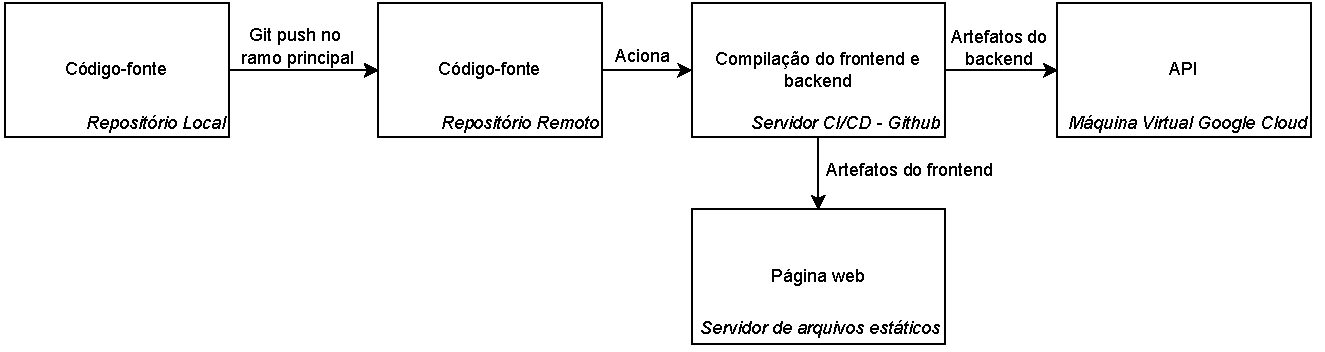
\includegraphics[width=\linewidth]{figures/ci-cd.pdf}
\end{figure}

A uso de práticas DevOps e pipelines de integração contínua e entrega contínua (CI/CD) com o GitHub no desenvolvimento do sistema de informação de um sistema inteligente para busca de imagens similares em astronomia oferece vantagens significativas em termos de automação, colaboração e qualidade do software. Este procedimento promove uma forma de integração entre desenvolvimento e operações, facilitando o gerenciamento eficiente de infraestrutura e aplicações.

Como mostra a Fig. \ref{fig:ci-cd}, as pipelines de CI/CD foram configuradas no GitHub para serem acionadas quando ocorrer alguma atualização no ramo principal, automatizando a execução de validação de código e implantação de novas versões do sistema. A pipeline compila o frontend e o backend, que são despachados automanticamente para servidores distintos. Os arquivos estáticos do frontend (HTML, CSS, JS, imagens) são enviados ao serviço de hospedagem de arquivos estáticos e páginas web do próprio Github. Já o backend é enviado à uma máquina virtual do Google Cloud.

Isso resultou em uma maior agilidade na entrega de atualizações. Além disso, a rastreabilidade e transparência proporcionadas pelo GitHub, combinadas com as práticas DevOps, asseguram um fluxo de trabalho organizado e escalável, que suporta tanto a evolução do sistema quanto a colaboração entre múltiplas equipes e pesquisadores.



\section{Considerações Finais do Capítulo}
\label{sec:conclusao-desenvolvimento}

O capítulo abordou detalhadamente o processo de desenvolvimento do sistema inteligente proposto, organizando-se em três seções principais que tratam dos conjuntos de dados (Seção \ref{sec:aquisicao}), do modelo de aprendizagem profunda (Seção \ref{sec:modelo}) e do sistema de informação (Seção \ref{sec:si}). Essa estrutura reflete a integração dos componentes fundamentais que compõem a solução.

Inicialmente, a Seção \ref{sec:aquisicao} descreve os métodos de aquisição, organização e pré-processamento dos dados utilizados no treinamento do modelo. Os rótulos são provenientes do Galaxy Zoo, e as imagens são oriundas do DESI Legacy Survey. Um ponto de destaque é o ajuste do campo de visão angular, que assegura que as características morfológicas de interesse das galáxias sejam corretamente capturadas. Essa etapa é complementada pela limpeza e pela organização dos conjuntos de treinamento, validação, teste e inferência, garantindo representatividade e evitando viés nos resultados.

Em seguida, na Seção \ref{sec:modelo}, são apresentadas as etapas de desenvolvimento do modelo de aprendizagem profunda, incluindo o aumento de dados, a escolha das arquiteturas de rede neural e o ajuste de hiperparâmetros. Modelos como EfficientNet e DenseNet são explorados devido à sua eficiência em capturar padrões visuais complexos. Além disso, são discutidas métricas de avaliação, como a métrica mAP (mean Average Precision), que assegura a robustez e a precisão do modelo na tarefa de recuperação de imagens baseadas em similaridade visual.

A Seção \ref{sec:si} aborda a implementação dos componentes do backend, frontend e banco de dados. O sistema foi projetado para suportar a indexação eficiente de embeddings e realizar buscas rápidas por similaridade visual. Tecnologias como PostgreSQL e pipelines DevOps foram empregadas para garantir desempenho, escalabilidade e integração contínua. O frontend oferece uma interface intuitiva, permitindo aos usuários interagir facilmente com os dados e os resultados do sistema.

Por fim, a Fig. \ref{fig:diagrama-completo} sumariza todas as etapas desenvolvidas na solução. Os resultados obtidos serão abordados no próximo capítulo.

\begin{figure}[!ht]
  \centering
  \caption{Sumário do desenvolvimento do projeto}
  \label{fig:diagrama-completo}
  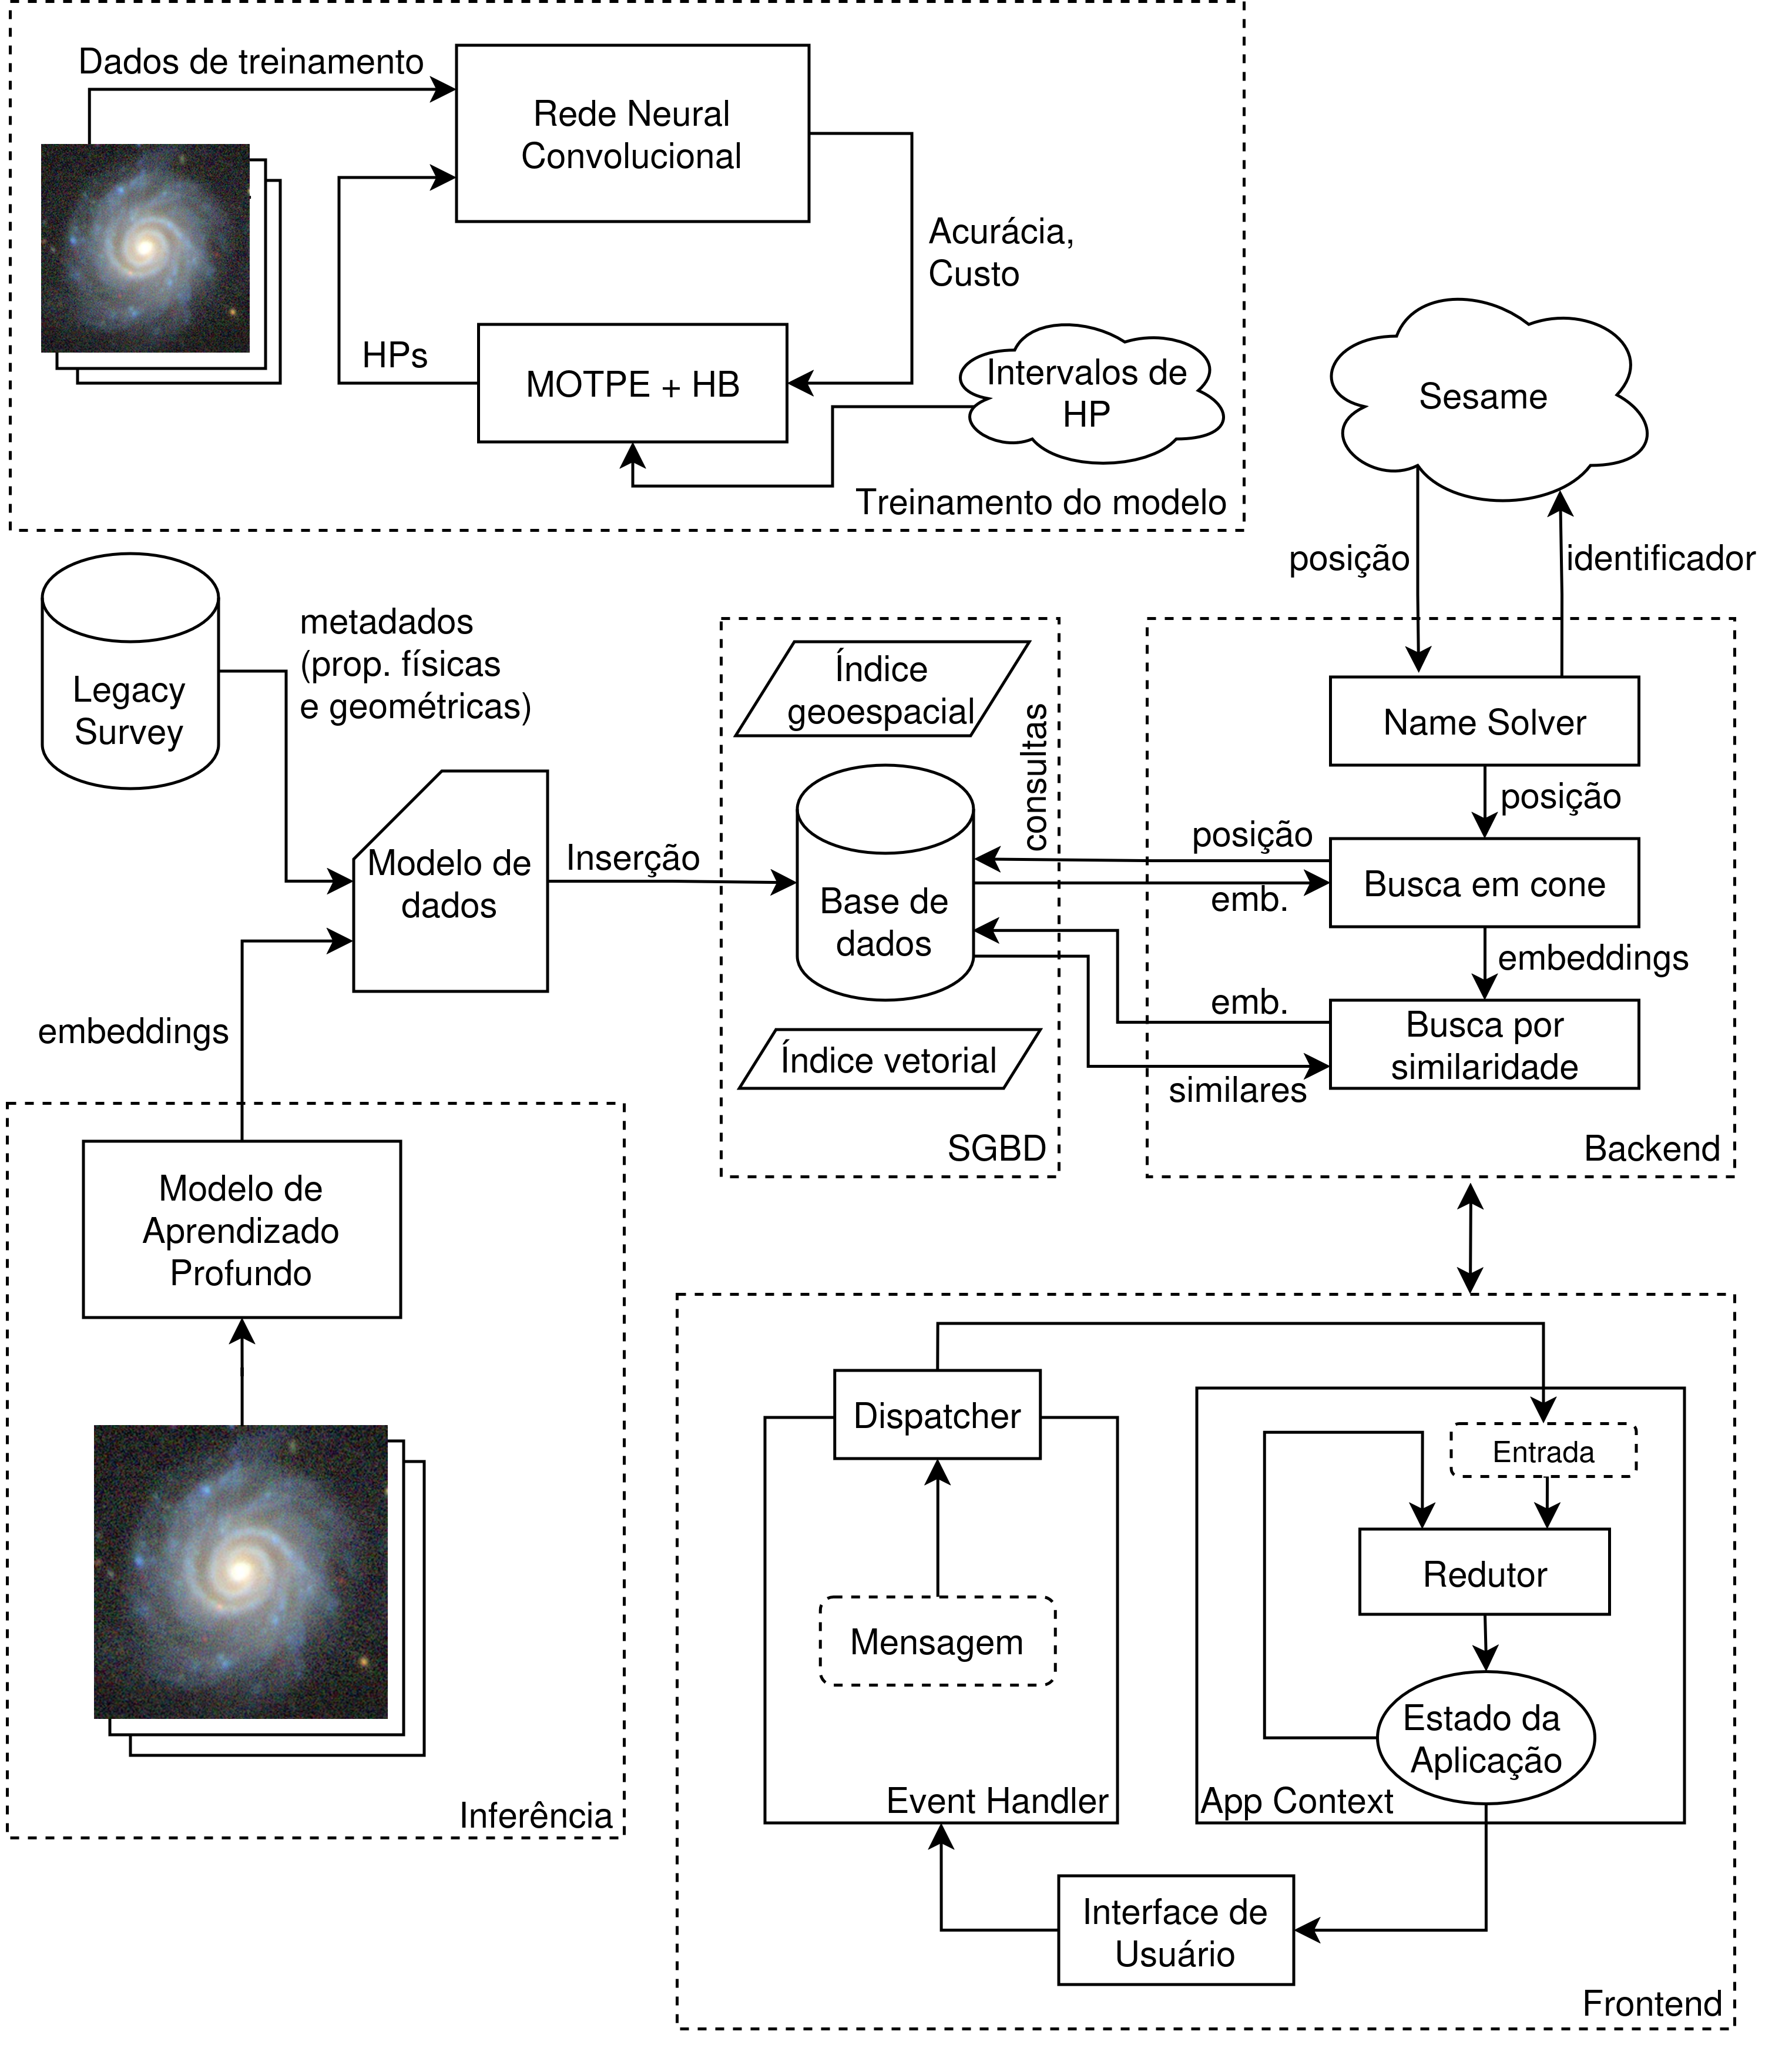
\includegraphics[width=\linewidth]{figures/full_diagram.png}
\end{figure}

\chaptersep


% \section{Conclusão do Capítulo}
